\chapterimage{Week3Clarifier1.jpg}
\chapter{Water Treatment}



\begin{table}[H]
\begin{tabular}{| m{1cm} | m{1cm} | m{12cm} |}
\hline
\multicolumn{3}{|l|}{\textbf{Expected   Range of Knowledge for Water Treatment}}                                                                         \\ \hline
\multicolumn{3}{|l|}{\textit{Water   Distribution System Operator License Exams}}                                                                        \\ \hline
\multicolumn{1}{l|}{} & \multicolumn{1}{l|}{D2-D5} & Ability to recognize   normal operation of in-line sensors                                 \\ \cline{2-3} 
\multicolumn{1}{l|}{} & \multicolumn{1}{l|}{D2-D5} & Ability to   troubleshoot a chemical feeder                                                \\ \cline{2-3} 
\multicolumn{1}{l|}{} & \multicolumn{1}{l|}{D2-D5} & Knowledge of analysis   methods                                                            \\ \cline{2-3} 
\multicolumn{1}{l|}{} & \multicolumn{1}{l|}{D2-D5} & Knowledge of chemical   feeder components                                                  \\ \cline{2-3} 
\multicolumn{1}{l|}{} & \multicolumn{1}{l|}{D2-D5} & Knowledge of chemical   feeder types                                                       \\ \cline{2-3} 
\multicolumn{1}{l|}{} & \multicolumn{1}{l|}{D2-D5} & Knowledge of required   reagents and standards                                             \\ \cline{2-3} 
\multicolumn{1}{l|}{} & \multicolumn{1}{l|}{D3-D5} & Knowledge of   corrosion control techniques                                                \\ \cline{2-3} 
\multicolumn{1}{l|}{} & \multicolumn{1}{l|}{D3-D5} & Knowledge of   principles of operation of cathodic protection devices                      \\ \hline
\multicolumn{3}{|l|}{Water   Treatment Operator License Exams}                                                                                  \\ \hline
\multicolumn{1}{l|}{} & \multicolumn{1}{l|}{T1-T4} & Ability to calculate   a dosage for a chemical feeder                                      \\ \cline{2-3} 
\multicolumn{1}{l|}{} & \multicolumn{1}{l|}{T1-T4} & Ability to calibrate   and adjust a chemical feeder pump                                   \\ \cline{2-3} 
\multicolumn{1}{l|}{} & \multicolumn{1}{l|}{T1-T4} & Ability to operate a   chemical feeder system                                              \\ \cline{2-3} 
\multicolumn{1}{l|}{} & \multicolumn{1}{l|}{T1-T4} & Ability to replace   components of a chemical feeder system                                \\ \cline{2-3} 
\multicolumn{1}{l|}{} & \multicolumn{1}{l|}{T1-T4} & Ability to set proper   chemical feed rate                                                 \\ \cline{2-3} 
\multicolumn{1}{l|}{} & \multicolumn{1}{l|}{T1-T4} & Knowledge of chemical   feeder calibration and adjustment                                  \\ \cline{2-3} 
\multicolumn{1}{l|}{} & \multicolumn{1}{l|}{T1-T4} & Knowledge of the   components of chemical feeder systems                                   \\ \cline{2-3} 
\multicolumn{1}{l|}{} & \multicolumn{1}{l|}{T1-T4} & Knowledge of the   operation of chemical feeder systems                                    \\ \cline{2-3} 
\multicolumn{1}{l|}{} & \multicolumn{1}{l|}{T1-T4} & Knowledge of basic   unit processes used in treating drinking water                        \\ \cline{2-3} 
\multicolumn{1}{l|}{} & \multicolumn{1}{l|}{T1-T4} & Knowledge of   corrective actions to take when regulations are violated                    \\ \cline{2-3} 
\multicolumn{1}{l|}{} & \multicolumn{1}{l|}{T2-T4} & Knowledge of   pretreatment procedures                                                     \\ \cline{2-3} 
\multicolumn{1}{l|}{} & \multicolumn{1}{l|}{T2-T4} & Knowledge of head   loss effects on filters                                                \\ \cline{2-3} 
\multicolumn{1}{l|}{} & \multicolumn{1}{l|}{T2-T4} & Knowledge of filter   surface washing methods                                              \\ \cline{2-3} 
\multicolumn{1}{l|}{} & \multicolumn{1}{l|}{T2-T4} & Knowledge of   filtration mechanisms (absorption, adsorption)                              \\ \cline{2-3} 
\multicolumn{1}{l|}{} & \multicolumn{1}{l|}{T2-T4} & Ability to choose an   appropriate disinfectant for a specific microbial problem           \\ \cline{2-3} 
\end{tabular}
\end{table}
\newpage




\begin{table}[H]
\begin{tabular}{| m{1cm} | m{1cm} | m{12cm} |}
\hline
\multicolumn{3}{|l|}{\textbf{Expected   Range of Knowledge for Water Treatment}}                                                                         \\ \hline
\multicolumn{3}{|l|}{\textit{Water   Treatment Operator License Exams (Continued)}}                                                                        \\ \hline
\multicolumn{1}{l|}{} & \multicolumn{1}{l|}{T2-T4} & Knowledge of   chloramine chemistry                                                        \\ \cline{2-3} 
\multicolumn{1}{l|}{} & \multicolumn{1}{l|}{T2-T4} & Knowledge of   disinfectant byproduct reduction procedures                                 \\ \cline{2-3} 
\multicolumn{1}{l|}{} & \multicolumn{1}{l|}{T2-T4} & Knowledge of   TOC/Disinfection byproduct correlation                                      \\ \cline{2-3} 
\multicolumn{1}{l|}{} & \multicolumn{1}{l|}{T2-T4} & Knowledge of   corrosion reduction methods                                                 \\ \cline{2-3} 
\multicolumn{1}{l|}{} & \multicolumn{1}{l|}{T2-T4} & Knowledge of Best   Available Technology (BAT) for common water contaminants               \\ \cline{2-3} 
\multicolumn{1}{l|}{} & \multicolumn{1}{l|}{T2-T4} & Knowledge of   effective removal techniques for common contaminants                        \\ \cline{2-3} 
\multicolumn{1}{l|}{} & \multicolumn{1}{l|}{T2-T4} & Knowledge of hardness   removal processes                                                  \\ \cline{2-3} 
\multicolumn{1}{l|}{} & \multicolumn{1}{l|}{T2-T4} & Knowledge of the   components of on-line analyzers                                         \\ \cline{2-3} 
\multicolumn{1}{l|}{} & \multicolumn{1}{l|}{T2-T4} & Ability to calculate   daily filter production                                             \\ \cline{2-3} 
\multicolumn{1}{l|}{} & \multicolumn{1}{l|}{T2-T4} & Ability to calculate   filter backwash rate                                                \\ \cline{2-3} 
\multicolumn{1}{l|}{} & \multicolumn{1}{l|}{T2-T4} & Ability to calculate   a CT value                                                          \\ \cline{2-3} 
\multicolumn{1}{l|}{} & \multicolumn{1}{l|}{T3-T4} & Ability to recognize   and correct problems in gravity filters                             \\ \cline{2-3} 
\multicolumn{1}{l|}{} & \multicolumn{1}{l|}{T3-T4} & Ability to recognize   and correct problems in multimedia filters                          \\ \cline{2-3} 
\multicolumn{1}{l|}{} & \multicolumn{1}{l|}{T3-T4} & Knowledge of backwash   sequencing                                                         \\ \cline{2-3} 
\multicolumn{1}{l|}{} & \multicolumn{1}{l|}{T3-T4} & Knowledge of filter   media types and uses                                                 \\ \cline{2-3} 
\multicolumn{1}{l|}{} & \multicolumn{1}{l|}{T3-T4} & Knowledge of maximum   filtration rates                                                    \\ \cline{2-3} 
\multicolumn{1}{l|}{} & \multicolumn{1}{l|}{T3-T4} & Knowledge of normal   and abnormal filter media conditions                                 \\ \cline{2-3} 
\multicolumn{1}{l|}{} & \multicolumn{1}{l|}{T3-T4} & Ability to calculate   filter media volume and capacity                                    \\ \cline{2-3} 
\multicolumn{1}{l|}{} & \multicolumn{1}{l|}{T3-T4} & Knowledge of iron and   manganese removal techniques                                       \\ \cline{2-3} 
\multicolumn{1}{l|}{} & \multicolumn{1}{l|}{T3-T4} & Knowledge of the   aeration process                                                        \\ \cline{2-3} 
\multicolumn{1}{l|}{} & \multicolumn{1}{l|}{T3-T4} & Knowledge of the   operation of blowers and compressors                                    \\ \cline{2-3} 
\multicolumn{1}{l|}{} & \multicolumn{1}{l|}{T3-T4} & Ability to   discriminate between normal and abnormal operation of blowers and compressors \\ \cline{2-3} 
\multicolumn{1}{l|}{} & \multicolumn{1}{l|}{T3-T4} & Knowledge of the   components of pressure gauges                                           \\ \cline{2-3} 
\multicolumn{1}{l|}{} & \multicolumn{1}{l|}{T3-T4} & Ability to recognize   analytical interferences in on-line analyzers                       \\ \cline{2-3} 
\multicolumn{1}{l|}{} & \multicolumn{1}{l|}{T3-T4} & Ability to repair or   replace defective parts of on-line analyzers                        \\ \cline{2-3} 
\multicolumn{1}{l|}{} & \multicolumn{1}{l|}{T3-T4} & Knowledge of the   operation of on-line analyzers                                          \\ \cline{2-3} 
\multicolumn{1}{l|}{} & \multicolumn{1}{l|}{T3-T4} & Knowledge of the   operation of an electrical generator                                    \\ \cline{2-3} 
\multicolumn{1}{l|}{} & \multicolumn{1}{l|}{T3-T4} & Knowledge of the   components of an electrical generator                                   \\ \cline{2-3} 
\multicolumn{1}{l|}{} & \multicolumn{1}{l|}{T4}    & Ability to conduct a   comprehensive performance evaluation of a filter                    \\ \cline{2-3} 
\multicolumn{1}{l|}{} & \multicolumn{1}{l|}{T4}    & Ability to operate an   air scour system                                                   \\ \cline{2-3} 
\multicolumn{1}{l|}{} & \multicolumn{1}{l|}{T4}    & Ability to perform a   filter assessment surveillance program                              \\ \cline{2-3} 
\multicolumn{1}{l|}{} & \multicolumn{1}{l|}{T4}    & Ability to perform a   filter profile analysis                                             \\ \cline{2-3} 
\multicolumn{1}{l|}{} & \multicolumn{1}{l|}{T4}    & Ability to recognize   and correct problems in granular activated carbon filters           \\ \cline{2-3} 
\end{tabular}
\end{table}
\newpage


\begin{table}[H]
\begin{tabular}{| m{1cm} | m{1cm} | m{12cm} |}
\hline
\multicolumn{3}{|l|}{\textbf{Expected   Range of Knowledge for Water Treatment}}                                                                         \\ \hline
\multicolumn{3}{|l|}{\textit{Water   Treatment Operator License Exams (Continued)}}                                                                        \\ \hline
\multicolumn{1}{l|}{} & \multicolumn{1}{l|}{T4}    & Knowledge of air   scouring systems                                                        \\ \cline{2-3} 
\multicolumn{1}{l|}{} & \multicolumn{1}{l|}{T4}    & Knowledge of filter   media replacement requirements and techniques                        \\ \cline{2-3} 
\multicolumn{1}{l|}{} & \multicolumn{1}{l|}{T4}    & Knowledge of filter   porosity                                                             \\ \cline{2-3} 
\multicolumn{1}{l|}{} & \multicolumn{1}{l|}{T4}    & Ability to choose the   proper corrosion control chemical for a specific problem           \\ \cline{2-3} 
\multicolumn{1}{l|}{} & \multicolumn{1}{l|}{T4}    & Knowledge   fluoridation chemicals                                                         \\ \cline{2-3} 
\multicolumn{1}{l|}{} & \multicolumn{1}{l|}{T4}    & Knowledge of fluoride   chemistry                                                          \\ \cline{2-3} 
\multicolumn{1}{l|}{} & \multicolumn{1}{l|}{T4}    & Knowledge of chemical   oxidation techniques and uses                                      \\ \cline{2-3} 
\multicolumn{1}{l|}{} & \multicolumn{1}{l|}{T4}    & Knowledge of granular   activated carbon (GAC)                                             \\ \cline{2-3} 
\multicolumn{1}{l|}{} & \multicolumn{1}{l|}{T4}    & Knowledge of nitrate   removal processes                                                   \\ \cline{2-3} 
\multicolumn{1}{l|}{} & \multicolumn{1}{l|}{T4}    & Ability to replace   components of blowers and compressors                                 \\ \cline{2-3} 
\multicolumn{1}{l|}{} & \multicolumn{1}{l|}{T4}    & Knowledge of the   components of blowers and compressors                                   \\ \cline{2-3} 
\end{tabular}
\end{table}
\newpage





\section{Background}\index{Background}
\begin{itemize}
\item Purpose of water treatment is to provide safe drinking water that does not contain objectionable taste, odor or color and provide adequate quantities of water for domestic, commercial, industrial and fire protection needs.

\item Even though U.S. tap water supplies are considered to be among the safest in the world, water contamination can still occur. There are many possible sources of contamination, including:
\begin{itemize}
\item Sewage releases
\item Naturally occurring chemicals and minerals (for example, arsenic, radon, uranium)
\item Local land use practices (for example, fertilizers, pesticides, livestock, concentrated feeding operations)
\item Manufacturing processes (for example, heavy metals, cyanide)
\item Malfunctioning on-site wastewater treatment systems (for example, septic systems)
\item In addition, drinking water that is not properly treated or that travels through an improperly maintained distribution system (pipes) may also create conditions that increase risk of contamination.
\end{itemize}

\item Drinking water quality varies from place to place, depending on the condition of the source water from which it is drawn and the treatment it receives, but it must meet U.S. Environmental Protection Agency (\colorbox{pink}{EPA}) regulations. Community water systems follow the rules set forth by the Safe Drinking Water Act (\colorbox{pink}{SDWA}).

\item The level of treatment and treatment processes used are primarily dependent on the quality - level of contamination of the source water.

\item Generally speaking surface waters contain more contaminants compared to groundwater as surface waters are more exposed to contamination from runoffs etc.  
\item Although groundwaters are succeptible to contamination from seepage and soil percolation, the sediment layers help filter water naturally. 

\item The quantity and quality of surface water supplies vary more than groundwater, particularly seasonally.

\item The purpose of water treatment is to condition, modify, or remove undesirable impurities and to provide water that is safe, palatable, and acceptable to users. Some regulations state that if the contaminants listed under the various regulations are found in excess of the Maximum Contaminant Levels (\colorbox{pink}{MCLs}), the water must be treated to reduce the levels. 

\item The primary objective of the Surface Water Treatment Rule (\colorbox{pink}{SWTR}) of the SWDA is to control microbiological contamination - specifically pathogenic bacteria and parasites, specifically \textit{Giardia lamblia} and \textit{Giardia lamblia}.

\item Groundwater from a well or spring which is influenced by surface water - Groundwater Under Direct Influence of Surface Water (\colorbox{pink}{GWUDI}) is subjected to the SWTR based treatment requirements, regardless of the actual presence of contamination. If they exceed secondary MCLs established by EPA and the state, the water may have to be treated. 

\item If we assume that the water source used to feed a typical water supply system is groundwater, which is usually the case in the U.S., a number of common groundwater problems may require water treatment. Among these other problems are: bacteriological contamination, hydrogen sulfide odors, hard water, corrosive water,and iron and manganese.

\item Many states enforce their own drinking water standards that are at least as protective as EPA’s national standards. The SDWA rules include guidelines for drinking water quality, water testing schedules, and water testing methods.

\item Private wells, which are not regulated by the EPA, supply drinking water to over 15 million homes. Well owners are responsible for keeping their water clean and safe.

\item When water system officials find an issue with the drinking water supply (for example, that it has become contaminated), a water advisory may be issued to help protect the public’s health.

\item The presence of certain contaminants in our water can lead to health issues, including gastrointestinal illness, reproductive problems, and neurological disorders. Infants, young children, pregnant women, the elderly, and people with weakened immune systems may be especially at risk for illness.

\item All water produced by public water systems must be drinking water quality, even though only about 1\% of water produced is used for drinking and cooking.

\item Water may be treated differently in different communities depending on the quality of the source water that enters the treatment plant. The water that enters the treatment plant is most often either surface water or ground water. Surface water typically requires more treatment and filtration than ground water because lakes, rivers, and streams contain more sediment (sand, clay, silt, and other soil particles), germs, chemicals, and toxins than ground water.

\item Some water supplies may contain radionuclides (small radioactive particles), specific chemicals (such as nitrates), or toxins (such as those made by cyanobacteria). Specialized methods to control or remove these contaminants can also be part of water treatment.

Schematic of conventional water treatment:
\begin{enumerate}
\item Water is withdrawn from a lake, reservoir or river at the intake
\item It is screened to remove debris
\item Water then enters the flash mixing tank where coagulants and other chemicals are added
\item Then it is divided into the flocculation basin
\item After flocculation, the water enters the settling basins where solids are removed
\item Filtration then removes particles that are too small to settle by gravity
\item The water is disinfected using some form of chlorine
\item Other chemicals such as fluoride, phosphate corrosion inhibitors or pH adjustment chemicals may be added
\item After a minimum detention time, the water may be pumped to the distribution systems Other processes may occur, such as pre-oxidation or activated carbon treatment.
\end{enumerate}

\begin{figure}[h]
\begin{center}
\includegraphics[scale=0.5]{WaterTreatment_9-01}
\caption{Conventional Water Treatment}
\end{center}
\end{figure}

\item There are many treatment approaches when it comes to treating a range of problems that can occur in groundwater. Many of these methods use a combination of technologies. When considering the appropriate approach, it is important to note that each site should be treated case by case. Since every site offers a different history, background, and unique landscape. 

\section{Categories of Treatment Methods}\index{Categories of Treatment Methods}
Typical treatment methods used can be categorized as:

\begin{enumerate}
\item Biological\\
\begin{itemize}
\item Microbes based biological systems are used for nutrient and organic removals from drinking water
\item Typically the biological processes utilize the fixed biofilm - support medium on which the biomass is attached.
\item Some applications use suspended growth reactors where the biomass is suspended in the water being treated. 
\end{itemize}

\item Chemical\\
\begin{itemize}
\item Chemical oxidants are injected or mixed into groundwater to destroy contaminants upon contact. Chemical oxidants include oxygen gas, ozone, and other liquid chemicals.\\
\end{itemize}
\item Physical\\
Most common physical techniques are:\\
\begin{itemize}
\item Sedimentation:  Involves gravity settling of settleable particles by gravitational force from the water.
\item Filtration involves removal of pollutants by physical processes including straining, adsorbtion and absorption.
\item Dissolved air flotation or Degasification:  Utilizes pressurized air to remove dissolved gases is the process of removing dissolved gases from the water.

\end{itemize}



\end{enumerate}
\vspace{1cm}

\section{Source Management}\index{Source Management}
\begin{itemize}
\item When options are available, source management implies effectively managing water sources, to ensure the intake of best possible quality of water from a regulatory compliance and treatment optimization perspective.
\item Examples of source management include:
\begin{itemize}
\item For systems using lake or reservoir sources, selecting the optimum depth from which to draw water depending on the water quality during that time of year or for other reasons (e.g. algal bloom,
storm upsets, etc).
\item Systems that have multiple sources may consider blending or alternating surface and ground
water sources to attain the best blended raw water for compliance. If blended prior to treatment, all water must be treated to surface water standards.
\end{itemize}
\end{itemize}

\section{Surface Water Treatment Processes}\index{Surface Water Treatment Processes}
\subsection{Source Water Treatment}\index{Source Water Treatment}
\begin{itemize}
\item Source water treatment in reservoirs or lakes includes treatment to contain algae growth.
\item Algal bloom is a sudden large increase in algae caused by weather or by nutrients. 
\item Reasons for controlling algae:
\begin{itemize}
\item Taste and odor problems
\item Shortened filter runs
\item Changes in pH - increases during the day, decreases at night
\item When algae dies, causes depletion of dissolved oxygen (DO)
\item Organic loading which is DBP pre-cursor resulting in TTHMs.
\end{itemize}
\item Algaecide such as blue stone, copper sulfate (CuSO$_4$) is used to control algae. 
\item Action level for copper is 1.3 mg/L·	·

\item Copper sulfate dose is usually specified in terms of pounds/acre. 
\item 5.4 lbs/acre is common dosage - the rate of application is based on the surface area of the reservoir not the volume
\item For water with alkalinify of higher than 150 mg/L, citric acid has to be mixed with CuSO$_4$ for it to be effective
\item Methods for dosing CuSO$_4$:
\begin{itemize}
\item Application of copper sulfate:
\item Dragging burlap bags behind a boat. Rate of application is controlled by the speed at which boat is traveling. ·
\item Using a hopper mounted on a boat
\item Spraying solution from a boat
\item Aerial spraying 
\end{itemize}

\end{itemize}
\subsection{Screening}\index{Screening}
\begin{itemize}
\item River water (the source of water used in our discussion) frequently contains suspended and floating debris varying in size from small rags to logs. Screening is usually the first major step where by large and suspended debris in the source water including sticks, leaves etc. is removed from the water before it enters the plant. 
\item Removing these solids is primarily to prevent damage to downstream equipment including pumps, prevent deposition of this debris in open channels or pipes, or in treatment processes.
\item The most important criteria used in the selection of a particular screening system for are the screen opening size and flow rate. Other important criteria include costs related to operation and equipment, plant hydraulics, debris handling requirements, and operator qualifications and availability. 
\item Depending on the characteristics of the source water, variety of screening devices including trash rakes, bar screens and wire mesh screens may be used. Very small screens can be used to screen out elements including algae in the water.
\item Typical screening devices used include:
\begin{itemize}
\item Trash Screens (Rakes) - used to remove rough or large debris.  The bar spacing in Rakes range from 1.5 to 4 inches.
\item Traveling Water Screens (Bandscreens) - these are placed in a channel of flowing water to remove floating or suspended debris.
\begin{figure}[h]
\begin{center}
\includegraphics[scale=0.25]{TrashRakes}
\captionof{figure}{Trash Rake}
\includegraphics[scale=0.5]{TravellingScreen}
\captionof{figure}{Band Screen}
\end{center}
\end{figure}
\end{itemize}

%\begin{center}
%\tcbox{\includegraphics[width=6cm]{TrashRakes}}
%Trash Rakes
%\tcbox{\includegraphics[width=6cm]{TravellingScreen}}
%\end{center}


\end{itemize}

\subsection{Coagulation and Flocculation}\index{Coagulation and Flocculation}
\begin{itemize}
\item A significant amount of suspended particles in the raw water are too small to be filtered or settled out in the sedimentation basin.  These particles, termed as non-settleable solids include organic matter, silt, clay.
\item These particles impart turbidity and color to the water and may harbor pathogens and typically carry a negative electrostatic charge on its surface.  The like surface charge on these particles cause electrostatic repulsion (particles keep bouncing off one another) which makes these particles difficult to settle. 
\item Coagulation and flocculation are sequential processes both of which involve chemical addition.
\item For coagulation, either metal salt type coagulant - typically an aluminum salt such as alum or aluminum sulfate or an iron salt such as ferric or ferrous chloride or sulfate, polyaluminum chloride or a organic coagulant such as polyDADMAC or polyamine is used. The coagulant helps coalesce the non-settleable solids into larger particles.
\item Sodium aluminate is often used as an aide to alum coagulation particularly for cold water and during lime softening.
\item Coagulation is affected by changes in the water's pH, alkalinity, temperature, time, velocity and zeta potential.

\item The effectiveness of a coagulant is generally pH dependent. Water with a color will coagulate better at low pH (4.4-6) with alum.

\item Alkalinity is needed to provide anions, such as (OH) for forming insoluble compounds to precipitate them out. It could be naturally present in the water or needed to be added as hydroxides, carbonates, or bicarbonates.  Generally 1 part alum uses 0.5 parts alkalinity for proper coagulation.

\item The higher the temperature, the faster the reaction, and the more effective is the coagulation. Winter temperature will slow down the reaction rate

\item The coagulation process requires rapid mixing of the water upon the addition of the coagulant followed by a sufficient contact time prior to the flocculation step.
\item The flocculant which is added after the coagulation step is to make even larger, more compact and settleable - \colorbox{lime}{floc}, from the coagulated solids.
\item Flocculants are typically long chain organic compounds - polymers with charged end groups.  \colorbox{lime}{anionic polymers} have a negative end group whereas \colorbox{lime}{nonionic polymers} have balanced - positive and negative end groups.
\item For the floc formed to remain intact, the polymer is gently "folded in" with the coagulated solids.  The flocculation is done in a flocculator which have a detention time of 5 -30 minutes and the water is mixed with the polymer using slow moving paddles.
\item Coagulant aids - chemicals which aid in the coagulation process and strengthening the flow include:
\begin{itemize}
\item Alakalinity enahncers - lime, Soda ash, caustic soda and sodium bicarbonate.
\item Weighting agents - calcimu carbonate and bentonite clay.  These are used in waters which are low in tubidity and high in color which under normal condition would have formed weak, slow settlling floc.
\item Activated sililca - sodium silicate activated by hypochlorous acid is often used as a coagulant aid with alum.
\end{itemize}


\end{itemize}

\item These will usually be used in conjunction with a primary coagulant such as ferric chloride, ferric sulfate, or alum.

\vspace{0.6cm}
\hspace{3.8 cm} \textbf{Coagulation-Flocculation Schematic}\\
\vspace{0.6cm}
\includegraphics[scale=.13]{CEPTInitial} \hspace{0.7 cm}\includegraphics[scale=.13]{CEPTCoagulation}\hspace{0.7 cm}
\includegraphics[scale=.13]{CEPTFlocculation}\\
\hspace{0.8cm} \textbf{Untreated Water}\hspace{2.4 cm}\textbf{Coagulation}\hspace{3 cm}\textbf{Flocculation}\\	

\item Determining the amount and type of coagulant used changes based on a variety of process conditions and quality of water. For example, a heavy rain will greatly impact the influent, or raw, water in a municipal treatment plant.

\item The jar test is a standard method in which various amounts of coagulant and flocculation times are tested on a raw water sample. There are multiple samples to test before implementation into a larger volume of the water treatment process.

\begin{figure}[h]
\begin{center}
\includegraphics[scale=0.2]{JarTest}
\caption{Jar Testing}
\end{center}
\end{figure}	

\end{itemize}
\subsection{Clarification/Sedimentation}\index{Clarification/Sedimentation}
\begin{itemize}
\item Clarification, or sedimentation, is the third step in conventional water treatment, after coagulation and flocculation and before filtration.
\item In the sedimentation basin the flocculated particles settle out under the influence of gravity.
\item In conventional sedimentation basins the solids drop out (settle) as the water slowly flows across the basin from the influent to effluent end.
\item Sedimentation basins are designed to create conditions in which the water flows very slowly through the basin, with minimal turbulence.
\item Conventional sedimentation basins are typically rectangular or cylindrical concrete or steel vessels which incorporate a horizontal flow of water.
\item To reduce the footprint of the conventional sedimentation basins, upflow-type clarifiers.
\item Synonyms:  primary treatment basin, primary clarifier, sedimentation basin, primaries, clarifier

	
		\item Primary treatment is after preliminary treatment and 				before secondary treatment
		\item Its two main objectives are: 
			\begin{itemize}
				\item Remove settleable solids
				\item Remove floatable solids
			\end{itemize}
		\item This is a physical process which relies on the physical 			properties - how heavy or light the suspended solids particles 		are to effect its separation
		\item Provides quiescent conditions for the influent 					wastewater for the heavier solids to settle and the lighter 			solids to float
		\item Removes settleable solids and floatables
		\item Settled solids are removed as sludge from the bottom of 			the clarifier
		\item Floatable solids including oil and grease are also 				removed, as scum from the surface\\
		\item The shape of the primary clarifier is either rectangular 		or circular
	
		\item Effective solids removal in the primary clarifiers will 			reduce the loading on the expensive secondary treatment 				process.
		\item The amount of solids removed during primary treatment 			may be enhanced by chemical addition - ferric or ferrous 				chloride as a coagulant and anionic polymer as the flocculant.  		This is called Chemically Enhanced Primary Treatment (CEPT).
\item \textbf{Typical Removal Rates:}\\
\begin{itemize}
\item \hspace{10mm} BOD removal – 25\% to 40\% and about 60\% with CEPT
\item \hspace{10mm} Suspended solids (SS) removal – 40\% to 60\% and about 75\% with CEPT
\item \hspace{10mm} Settleable Solids removal - $>$90\%
\end{itemize}
\end{itemize}
\clearpage
			\begin{center}
				\includegraphics[scale=0.9]{RectangularClarifier}\\
				Cross section of a Rectangular Clarifier\\

				\includegraphics[scale=0.1]{Blank}\\
				\includegraphics[scale=0.6]{CircularClarifierAI}\\
				Schematic cross section of a circular clarifier\\
				\includegraphics[scale=0.1]{Blank}\\
				\includegraphics[scale=0.5]{CircularClarifier3}\\
				Cross section of a circular clarifier\\
			\end{center}
				\includegraphics[scale=0.03]{Blank}\\


\section{Clarifier Zones}\index{Clarifier Zones}
				
\subsection{Inlet Zone}\index{Inlet Zone}		
				\begin{itemize}
					\item Inlet Zone is where the water enters the end 					of a rectangular tank, or the center of a circular 					or square tank.
					\item The Inlet Zone is designed to accomplish two 					objectives:
						\begin{enumerate}
							\item Reduce the velocity (dissipate 									energy in the incoming water)
							\item Distribute the flow evenly
						\end{enumerate}
					\item The inlet zone is equipped with a baffle.  					Inlet baffle reduces the velocity of the 							influent flow, prevent short circuiting which 							could cause solids being carried over to secondary 					treatment.  
						\begin{itemize}
							\item Circular tanks are equipped with a 								collar-type circular baffle that directs 								the water down as it enters the center of 								the tank.
							\item Rectangular tanks will have a plate 								baffle in front of the opening for the 									wastewater flow into the clarifier and 									another baffle just upstream - a 										perforated wall or a picket fence type 									baffle that spreads the water laterally 								across the inlet end of the tank.\\

\begin{figure}[h!]
  \centering
  \begin{subfigure}[b]{0.4\linewidth}
    \includegraphics[width=0.8\linewidth]{InfluentBaffle}
    \caption{Rectangular clarifier influent baffle}
  \end{subfigure}
  \hspace{1cm}
  \begin{subfigure}[b]{0.4\linewidth}
    \includegraphics[width=\linewidth]{CircularClarifierInfluentBaffle}
    \caption{Circular clarifier influent baffle}
  \end{subfigure}
\end{figure}	
	
%							\begin{center}
%							\includegraphics[scale=0.65]												{InfluentBaffle}\\
%							Rectangular clarifier influent baffle
%							\end{center}
%							
%														\begin{center}
%							\includegraphics[scale=0.65]												{CircularClarifierInfluentBaffle}\\
%							Circular clarifier influent baffle
%							\end{center}	
						\end{itemize}
				\end{itemize}

\subsection{Settling Zone}\index{Settling Zone}
			\begin{itemize}
				\item This is the largest portion of the tank where 					solids settle.
				\item The water velocity is reduced to 0.03-0.05 fps 					and the detention time is about 1.5 to 2 hours. 
				\item A clarifier is said to be short circuiting if 					the velocity of the water is greater in some sections 					than in others. The water passing through the higher 					velocity region will have a reduced detention time and 				settleable solids will carry through with this water 					as it goes over the weir.  Short circuiting is 							prevented by appropriately designing inlet baffles and weir plates (at the Outlet Zone).
			\end{itemize}

\subsection{Sludge Zone}\index{Sludge Zone}
			\begin{itemize} 
				\item Sludge zone is the bottom of the tank where the 					settled sludge collects and compacts.
				\item Sludge blanket depth should be measured and 						sludge should be removed at least every shift. A 						desirable blanket depth is typically established and 					the sludge pumping rate and regimen is established to 					maintain that desired sludge blanket level.
				\item Sludge rakes push the sludge to one end or the 					center of the tank so that it can be pumped out. 
				\item The rake drive is usually equipped with a torque 				indicator. A shear pin in the drive shaft will break 					to prevent damage to the gearbox or drive shaft. 
				\item Failure to remove sludge often enough will 						result in the sludge becoming septic releasing gas 						bubbles which hinders the sludge settling and also 						result in causing odor problems.
				\item The sludge from the primary clarifiers needs to 					be stabilized prior to its disposal.  The sludge 						(solids) from the primary clarifiers are mixed with 					the solids from the secondary treatment process and 					stabilized typically using a sludge digestion process. 
			\end{itemize}
\subsection{Skimming Zone}\index{Skimming Zone}

			\begin{itemize}
				\item The skimming zone is at the surface of the tank 					for scum removal
				\item Lighter solids and greases float to the surface 					of the clarifier as scum
				\item In Circular Clarifiers:  Floating matter is 						skimmed by a skimmer arm that is supported by the 						sludge rake and rotates with it around the tank. The 					floating matter is pushed over the beach plate by the 					wipers attached to the skimmer arm and into a scum box 				attached to the tank wall.\\
				\item In Rectangular Clarifiers:  The flights act as 							skimmers when the chain brings them to the surface and 				pushes the scum towards the scum troughs.  The scum 					trough may be designed to rotate (tip) periodically 					for the scum to flow in from the water surface.\\
							
				\item The scum collected from the primary clarifiers is sent 				to the digester for treatment along with the sludge 					removed.\\ 

				\vspace{1cm}
									\begin{center}
					\includegraphics[scale=0.06]{RotatingScumTrough}\\
					Rectangular clarifier scum trough\\
									\includegraphics[scale=0.02]{Blank}\\
				\end{center}	

				\item The flights in the rectangular clarifier are supported 				at the top by two parallel rails running along the 						length of the clarifier.\\
				\item There are wear plates (strips) installed at the 						clarifer bottom and on top of the rails to prevent the 				flights from riding directly on those surfaces.  To 					reduce friction, the flights have a wearing shoe 						attached.  
				\item Both the wear strip and the wearing shoe 					are disposable items and are replaced at fixed 							intervals.\\			
				\begin{center}
					\includegraphics[scale=0.07]												{RectangularClarifierComponents}\\
					Rectangular clarifier flights\\
				\end{center}						  
\end{itemize}
\subsection{Outlet Zone}\index{Outlet Zone}
			\begin{itemize}
				\item  This is the part of the clarifier where the 						settled water leaves to go to the secondary treatment 					processes.
				\item A channel called the effluent launder collects 					the effluent flow and directs it to the primary 						effluent piping. 
				\item Weirs are installed along the edge of the effluent launder channel to skim the water evenly off the surface of the tank. The most common type of effluent weir is a V-notch (or saw-tooth) weir.   A V-	notch weir is a plate that has notches, about 2-3 						inches deep, cut in it every 6-8 inches. If the weir is clean and level, it will remove water evenly all 					the way around the edge of the tank. This minimizes 					the upward velocities near the effluent launder and 					improves removal efficiencies. If the weir plate is not level or part of the weir becomes clogged with 				slime or debris, short-circuiting will result because 					more water will pass over the low side or the clean notches of the weir. Short-circuiting will cause poor 					settling and uneven sludge blanket buildup.
				\item In rectangular tanks the water leaves at the end 	opposite the influent.
												  
				\item In circular  tanks the water leaves at the edge of the tank.
				\item Also, in the circular clarifiers, an effluent baffle, just upstream of the weir, 					is installed to prevent floating solids from going 						over the weir.
\clearpage
				\begin{center}
					\includegraphics[scale=0.04]												{CircularClarifierComponents1}\\
					Circular clarifier skimmer arm, effluent baffle and v-notch weir\\
				\end{center}
				
			\vspace{0.8cm}
					\begin{center}
					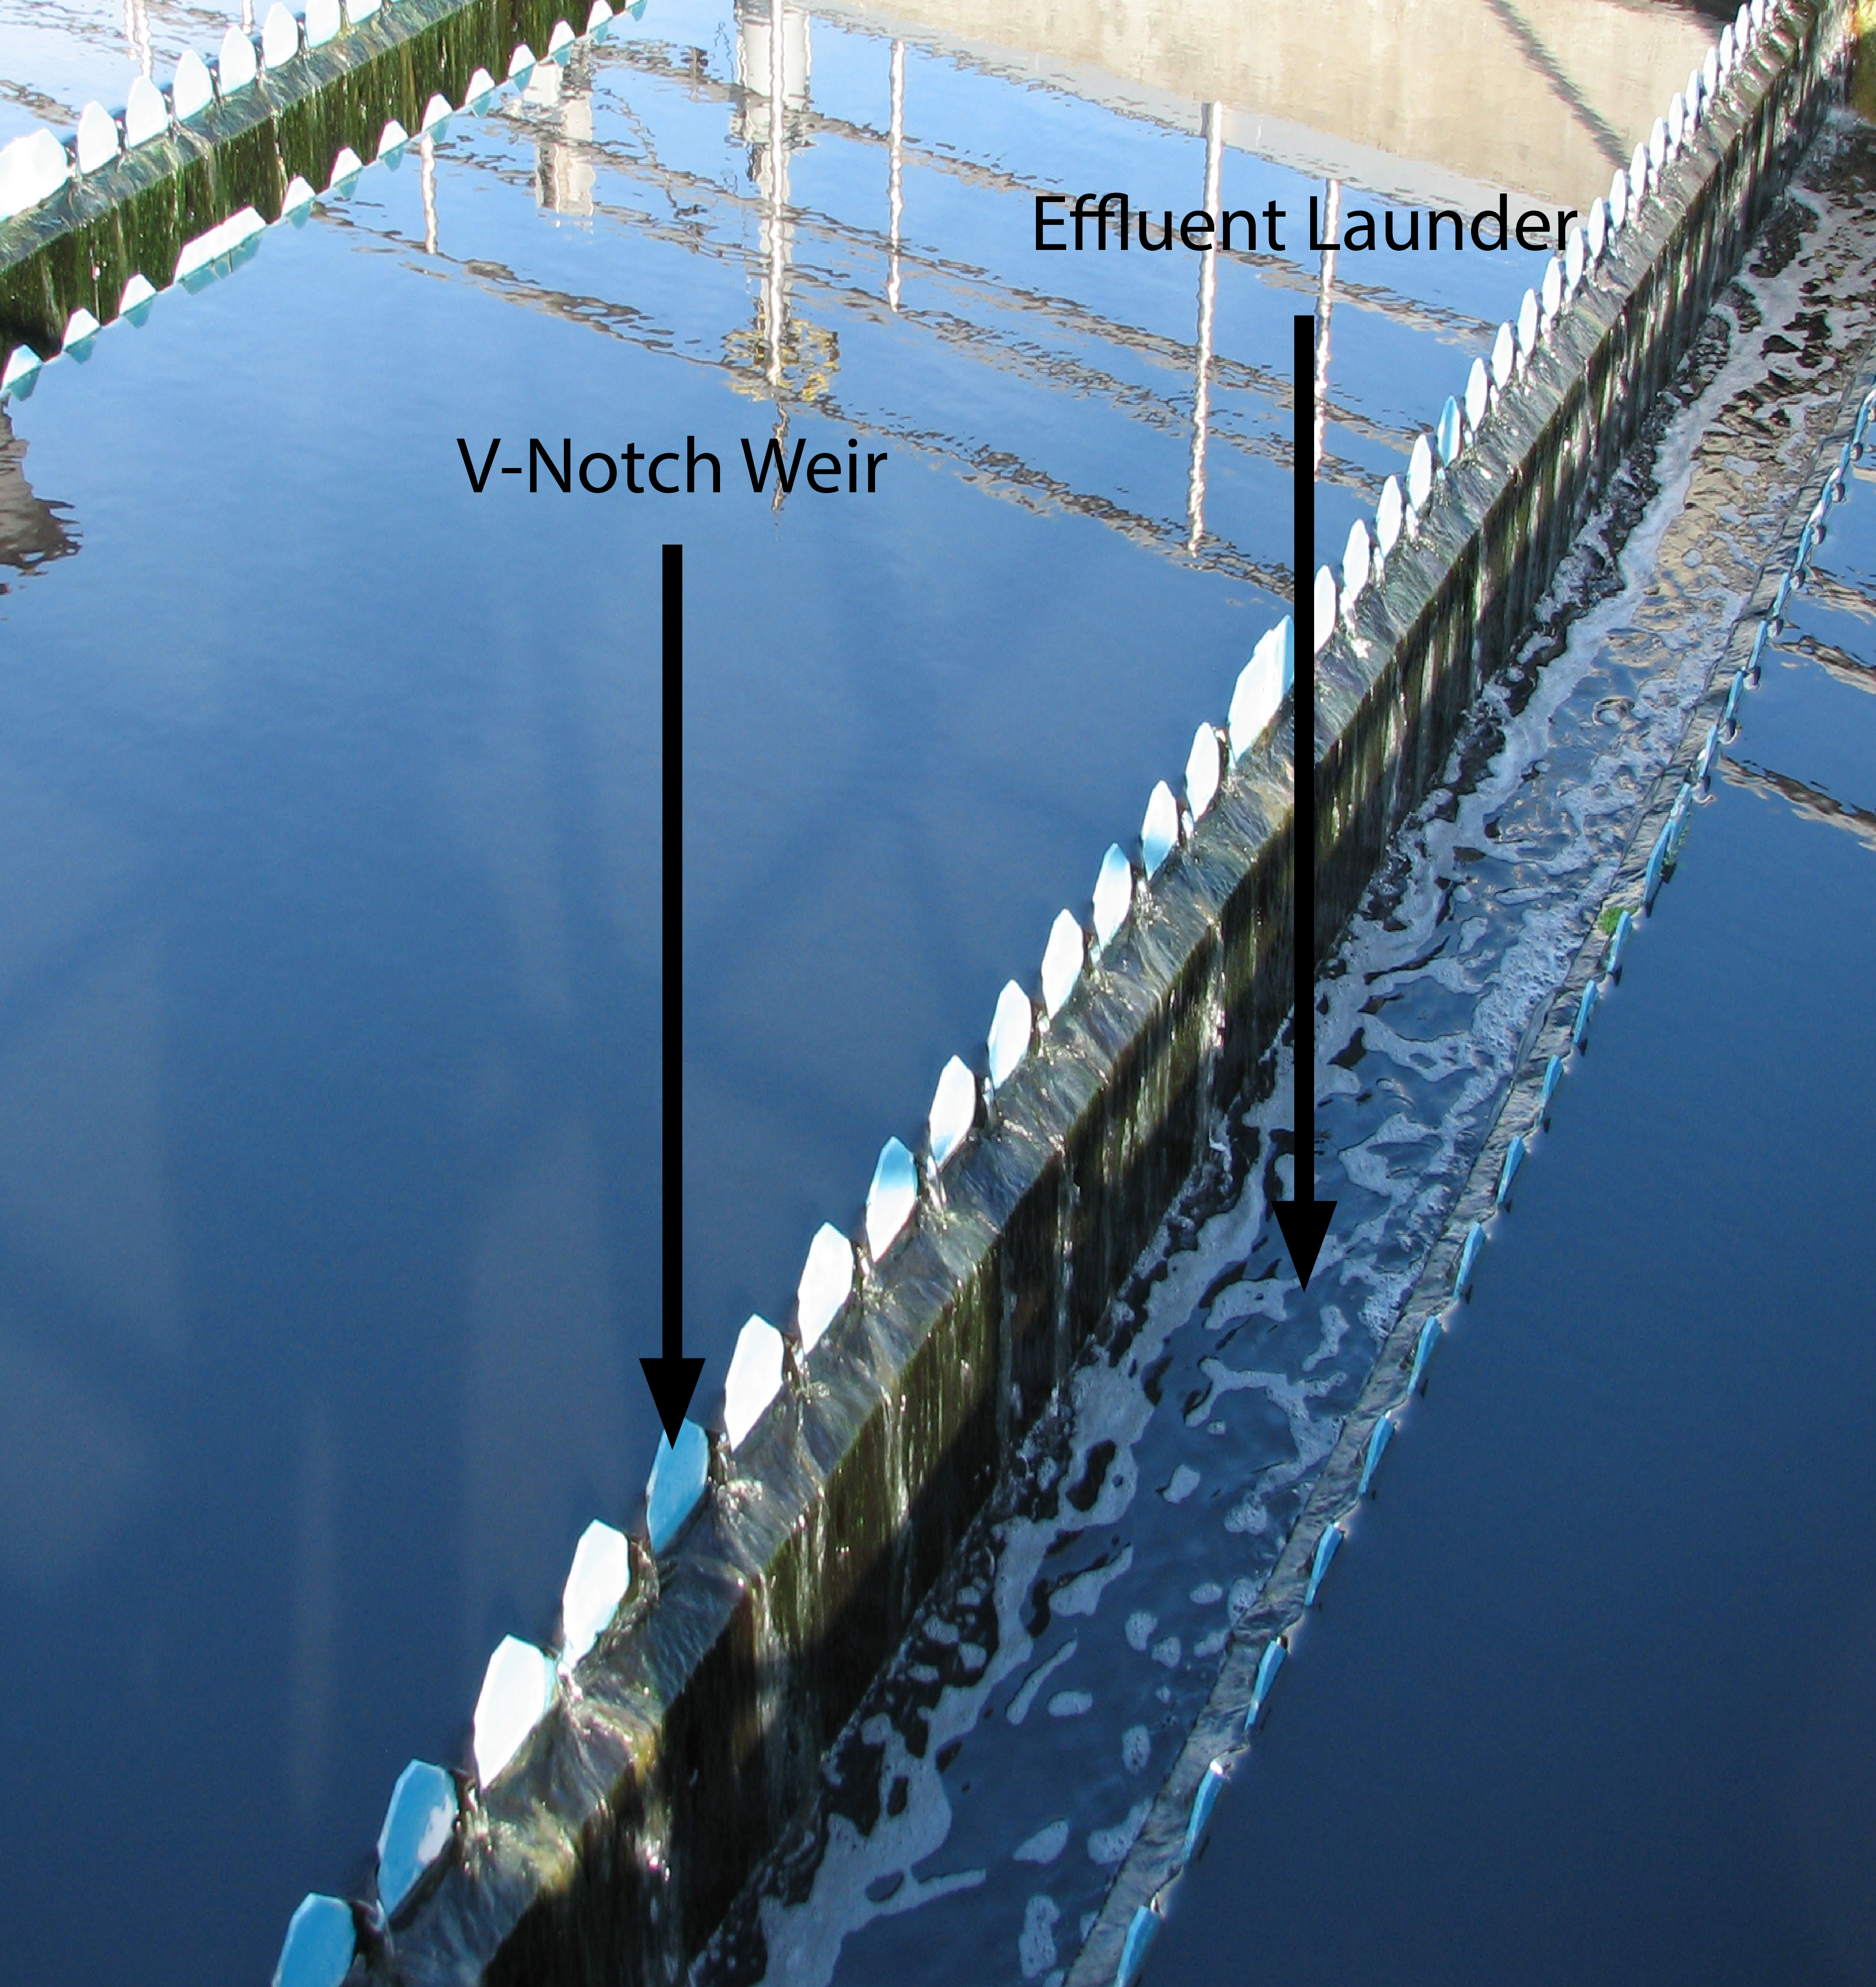
\includegraphics[scale=0.07]												{RectangularClarifierWeir}\\
					Rectangular clarifier v-notch weir and launder\\
				\end{center}			
												  
			\end{itemize}

\clearpage
\section{Sludge Pumping}\index{Sludge Pumping}

	\begin{itemize}
		\item The sludge pumping from the clarifier must be adequate 			to prevent sludge from going septic. Septic sludges are much 			more difficult to thicken or de-water and cause odor issues. 
		\item Primary sludge normally averages 4-6\% solids. 
		Generally positive displacement pumps are used for primary 				sludge
		\item The pumping cycles must be designed to provide the 				thickest sludge possible.
		\item Excessive pumping or pumping without building solids to 			build up leads to pumping thinner (more water) sludge.
	\end{itemize}


\section{Filtration}\index{Filtration}

\begin{figure}[h]
\begin{center}
\includegraphics[scale=1]{RapidFiltrationbyPretreatmentLevel1}
\caption{RapidFiltrationbyPretreatmentLevel 0.5}
\end{center}
\end{figure}

\begin{figure}[h]
\begin{center}
\includegraphics[scale=1]{DualMediaRapidFilter}
\caption{DualMediaRapidFilter 0.5}
\end{center}
\end{figure}

\begin{figure}[h]
\begin{center}
\includegraphics[scale=1]{SofteningLimeSoda}
\caption{SofteningLimeSoda 0.5}
\end{center}
\end{figure}

\begin{figure}[h]
\begin{center}
\includegraphics[scale=1]{MembraneFiltration}
\caption{MembraneFiltration 0.5}
\end{center}
\end{figure}
\subsubsection{Process Basics}\index{Process Basics}
\begin{itemize}
\item The SWTR requires the filtration of Surface water and ground water under the direct influence of surface water 
\item Slow sand filtration is one of a number of filtration technologies that can permit a water system to comply with the filtration requirements of the SWTR.
\item Filtration does not remove dissolved solids and by itelf is not effective for the removal of bacteria. Also, pre-treatment (example: coagulation/flocculation) and final disinfection are therefore needed. 
\item Conventional filtration is a four step treament process that consists of the treatment steps of coagualation, flocculation, sedimentation and rapid sand filtration. 
\item In filtration, solids are removed physically by:
\begin{itemize}
\item Straining – trapping particles, and 
\item Through adsorption.
\end{itemize}
\item Granular Bed and Pre-coat Filters are typically used for surface water treatment

\item Media in Granular Bed filter is comprised of one or a combination of the following:
\begin{itemize}
\item Sand
\item Anthracite
\item Granular activated carbon
\end{itemize}
\item Pre-coat filters use a thin layer of very fine medium such as diatomaceous earth.  Precoat filtration is used to remove very small particulate matter, oil particles, and even bacteria from water. This method is practical only for relatively small quantities of water which contain low concentrations of contaminants.
\item Filters can also be classified as:
\begin{itemize}
\item Gravity – open to atmosphere
\item Pressure – utilize a pressure vessel to contain the media
\end{itemize}
\item Gravity filters can be operated at different hydraulic rates
\begin{itemize}
\item Slow filters
\item Rapid filters
\end{itemize}
\item Filters can also be classified as:
\begin{itemize}
\item Depth filtration – solids are removed within the granular material.  Example: Rapid granular bed filter
\item Cake filtration – solids are removed on the entering face of the granular material.  Example: Precoat
\end{itemize}

\item Rapid sand filtration is the most common type of filtration used in water treatment. Whereas slow sand filtration is usually a feasible alternative for SWTR compliance only for small water systems with relatively high quality source water.
\item Filter media in a rapid sand filter refers to the granular material used to remove particles from the filter influent. 
\item Typical filter media in a rapid sand filter include sand (of course), and sometimes a “cap” of coal or granular activated carbon (GAC) placed on top of the sand media layer. 
\item Filters with a sand and coal/carbon cap are referred to as dual media filters. Some rapid sand filters also contain a thin layer of garnet sand. This layer also tends to improve filter performance.  
\item Filters with a layer of garnet sand are referred to as mixed media filters.
\item In a slow sand filter there is a  layer - \colorbox{lime}{Schmutzdecke} that develops on the top and is made up of microrganisms that feed on and break down organic material that is trapped on the surface of the filter. If the source water naturally contain low levels of nutrients, initial nutrient addition may be needed to develop this layer.

\begin{figure}[h]
\begin{center}
\includegraphics[scale=0.65]{SandFilter}\\
\captionof{figure}{Rapid Sand Filter}%\caption{}\\
\vspace{0.3cm}
\includegraphics[scale=0.65]{RapidSandFilter}\\
\captionof{figure}{Rapid Sand Filter}%\caption{}
\end{center}
\end{figure}
\end{itemize}


\subsubsection{Operation}\index{Operation}
\begin{itemize}
\item The removal mechanism in filtration involves straining – trapping larger particles and through adsorbtion where particles attach themselves to the filter media
\item Typical Filtration Rates:
\begin{itemize}
\item Slow Sand: 0.05 gpm/ft$^2$ - 3 feet sand
\item Rapid Sand: 2 gpm/ft$^2$ – 3 feet sand
\item Pressure filters: 3 gpm/ft$^2$
\item High Rate: 2-6 gpm/ft$^2$ – various media configurations
\end{itemize}

\item After a period of operation – filter cycle, the filter headloss increases because of the accumulation of the trapped solids.
\item Rapid filters are cleaned by backwashing using an upward, high-rate flow of water
\item Slow sand filters are cleaned by scrapping off the dirty layer from the surface.
\item The Schmutzdecke enhances the particulate removal.  As the Schmutzdecke develops, the filter performance – as measured by the turbidity typically improves as the filter run progresses.
\item Coagulation-flocculation is not required for cake filtration whereas chemical treatment is required for depth filtration.
\item Backwashing involves reversing the flow of water through the filter causing water to travel from the bottom of the filter to the top. 
\item Backwash is done at specific rates in order to most effectively remove the particulate material.  Backwashing process can be augmented by introducing low pressure air into the backwash line.
\item Backwash rates of 12-15 gpm/ft$^2$ or higher are common for sand, and rates for anthracite may range from 8 to 12 gpm/ft$^2$.
\item Wastewater used for the backwash is collected and removed from the filter. 






\item \textbf{Operational Problems}

Two common issues include:

\begin{itemize}

 

%black, blue, brown, cyan, darkgray, gray, green, lightgray, lime, magenta, olive, orange, pink, purple, red, teal, violet, white, yellow.

%\colorbox{declared-color}{text}

%\begin{tcolorbox}[width=\textwidth,colback={red},title={With true corners},outer arc=0mm,colupper=white]   

%   Air binding – vacuum generated due to higher water outflow than inflow causes violent upheaval impacting the media bed, gravel and/or underdrain.

    %\includegraphics[scale=0.5]{frogimage.png}

%\end{tcolorbox}   

\item \colorbox{lime}{Air Binding} – vacuum generated due to higher water outflow than inflow causes violent upheaval impacting the media bed, gravel and/or underdrain.

 

\item \colorbox{lime}{Mud balls} – these are formed as a result of inadequate backwashing and can cause the the filter to completely clogup.

\end{itemize}
\end{itemize}

\subsubsection{Greensand Filtration}\index{Greensand Filtration}
\begin{itemize}
\item Potassium Permanganate Oxidation and Manganese Greensand
\begin{itemize}
\item Utilizes greensand – a natural mineral (glauconite) coated with manganese dioxide as the filter media to remove iron and magnesium.
\item The Greensand catalyzes the oxidation of the dissolved iron and manganese forming solid particles which are filtered out.
\item Potassium permanganate is commonly used as the oxidant.
\end{itemize}
\end{itemize}
\subsubsection{Granulated activated carbon filter}\index{Granulated activated carbon filter}
\begin{itemize}
\item Granulated activated carbon filter\\
\vspace{0.3cm}
\begin{minipage}{.6\textwidth}
\begin{itemize}
\item Granulated Activated Carbon (\colorbox{pink}{GAC}) filters have a layer of activated carbon on top of anthracite or sand.
\item Activated carbon adsorbs various contaminants, such as tastes and odor-causing organics, THMs, and synthetic organics. 
\item GAC is lighter than sand or anthracite and has an effective size of 0.55 to 0.65 mm. \item These filters have the problem of losing some carbon during the backwashing; therefore backwashing is properly controlled to prevent the excessive loss of GAC. 
\item Commonly, backwashing causes 1 to 6 percent GAC loss per year.
\item Solids carbon blocks when used in lieu of granular carbon are effective in Cryptosporidium and Giardia removal.
\end{itemize}
\end{minipage}
 \begin{minipage}{0.5\textwidth}
        \centering
       \includegraphics[scale=0.7]{GAC}
    \end{minipage}\\

\end{itemize}.

\subsubsection{Math Problems}\index{Math Problems}
\begin{itemize}
\item \colorbox{lime}{Filter Flow Rates} – the flow rate expressed in gpm can be calculated from the total flow over certain time or vice-versa can be used for determining either the time it would take to process a certain flow or calculate the total flow.\\

 

 

\textbf{Example 1:}  A filter box is 20 ft by 30 ft (including the sand area). If the influent valve is shut, the water drops 3 inches per minute. What is the rate of filtration in MGD?\\

First let's write down what we are given:\\

 

Filter box = 20 ft x 30 ft Water drops = 3 in/min\\

Area = 20 ft x 30 ft = 600 ft2\\

Answer:  1122 gpm\\

 

 

\textbf{Example 2:}  The flow rate through a filter is 4.25 MGD. What is this flow rate expressed as gpm?\\

\vspace{0.2cm}

$Flow rate, gpm=\dfrac{Flow \enspace rate, \enspace gpd}{1440 \enspace min/day}$\\

\vspace{0.2cm}

Note:  We are assuming that the filter operated uniformly over that 24 hour period.\\

\vspace{0.3cm}

$Flow rate, gpm=\dfrac{4.25 \enspace \dfrac{\cancel{MG}}{\cancel{day}} *1,000,000 \enspace \dfrac{gal}{\cancel{MG}}}{1440\dfrac{min}{\cancel{day}}}=\boxed{2,951 \enspace gpm}$

 

\vspace{0.3cm}

\textbf{Example 3:}  At an average flow rate of 4000 gpm, how long of a filter run, in hours, would be required to produce 25 MG of filtered water?\\

\vspace{0.2cm}

$Flow \enspace rate \enspace (gpm)=\dfrac{Total \enspace flow \enspace (gal)}{Filter \enspace run \enspace time \enspace (min)}$

\vspace{0.3cm}

$\implies Filter \enspace run \enspace time \enspace (min)=\dfrac{Total \enspace flow \enspace (gal)}{Flow \enspace rate \enspace (gpm)}$\\

\vspace{0.3cm}

$\implies Filter \enspace run \enspace time \enspace (hr)=25 \enspace MG*\dfrac{1,000,000 \enspace \cancel{gal}}{MG}*\dfrac{\cancel{min}}{4,000 \enspace \cancel{gal}}*60 \enspace \dfrac{hr}{\cancel{min}}=\boxed{104 \enspace hrs}$

 

 

\item \colorbox{lime}{Filtration Rates} – It is the gallons of water filtered per minute through each square foot of filter area.  It generally ranging from 2 to $10 \mathrm{gpm} / \mathrm{ft}^{2}$.\\

Filtration rate is determined by the following equation:\\
$$
\text { Filtration rate, } \mathrm{gpm} / \mathrm{ft}^{2}=\frac{\text { Flow rate, } \mathrm{gpm}}{\text { Filter surface area, } \mathrm{ft}^{2}}
$$\\

\textbf{Example 1:} A filter $28 \mathrm{ft}$ long by $18 \mathrm{ft}$ wide treats a flow of $3.5 \mathrm{MGD}$. What is the filtration rate in gpm/ft ${ }^{2}$ ?\\

\vspace{0.2cm}
\textit{Approach:  The flow will need to be converted to gpm and the surface area calculated in feet.}\\

$\text{Filtration rate, } \mathrm{gpm} / \mathrm{ft}^{2} = 
\dfrac{
\dfrac{3.5 \enspace \cancel{MG}}{ \cancel{day}} * \dfrac{1,000,000 \enspace gal}{\cancel{MG}}
*\dfrac{\cancel{day}}{1440 \mathrm{ min}}}
{28 \enspace ft * 18 \enspace feet}= \boxed{4.8 \enspace gpm/ft^2}$\\
\vspace{0.2cm}
\textbf{Example 2:} A filter is $40 \mathrm{ft}$ long by $20 \mathrm{ft}$ wide. During a test of flow rate, the influent valve to the filter is closed for 6 minutes. The water level drop during this period is 16 inches. What is the filtration rate for the filter in $\mathrm{gpm} / \mathrm{ft}^{2}$ ?\\
\vspace{0.2cm}
\textit{Note:  The volume of the water dropped after the inlet valve was closed would be the filter flow rate.  Since the dimensions to calculate are in feet and inches, the volume needs to be converted from ft$^3$ to gallons}\\
\vspace{0.2cm}
$\text{Filtration rate, } \mathrm{gpm} / \mathrm{ft}^{2} = 
\dfrac{(
40 \mathrm{ ft}*20 \mathrm{ ft} * 16 \mathrm{\cancel{in}}*
\dfrac{ft}{12 \enspace \cancel{in}}
)
\cancel{ft^3}*7.48 \enspace 
\dfrac
{gal}
{\cancel{ft^3}}}
{40 \enspace ft * 20 \enspace feet}= \boxed{1.7\enspace gpm/ft^2}$\\

\item \colorbox{lime}{Backwashing Rates} - is the amount of water, in gallons, required for each backwash. This is analogous to the Filter Flow Rate.

\textbf{Example 1:}
A filter has the following dimensions: $30 \mathrm{ft}$ long by $20 \mathrm{ft}$ wide with a depth of 24 inches of filter media. Assuming that a backwash rate of $15 \mathrm{gal} / \mathrm{ft}^{2} / \mathrm{min}$ is recommended and 10 minutes of backwash is required, calculate the amount of water, in gallons, required for each backwash.

\textit{The backwashing rate given in $gal/ft^2/min$ will need to be converted into gallons by multiplying it with the area (to eliminate $ft^2$ and by the backwash time in minutes}

$ \text{Backwashing rate (gal)} = 15\dfrac{gal}{\cancel{ft^2}-\cancel{min}}*(30 \mathrm{ ft} \times 20 \mathrm{ ft})\cancel{ft^2}*10 \enspace \cancel{min}=\boxed{90,000 \enspace \text{gal}}$

\item \colorbox{lime}{Backwash Rinse Rates} - it is the upward velocity of the water during backwashing, expressed as in/min rise. To convert from $\mathrm{gpm} / \mathrm{ft}^{2}$ backwash rate to an in/min rise rate, use either of the following equations:

$$\text{ Backwash rinse rate, in/} \mathrm{min}=\frac{\text { Backwash rate, } \mathrm{gpm} / \mathrm{ft}^{2} \times 12 \mathrm{in} / \mathrm{ft}}{7.48 \mathrm{gal} / \mathrm{ft}^{3}}$$

\textbf{Example:1}
A filter $22 \mathrm{ft}$ long by $12 \mathrm{ft}$ wide has a backwash rate of $3260 \mathrm{gpm}$. What is this backwash rate expressed as a in/min rise?

$$\text{ Backwash rinse rate, in/} \mathrm{min}=\frac{\text { Backwash rate, } \mathrm{gpm} / \mathrm{ft}^{2} \times 12 \mathrm{in} / \mathrm{ft}}{7.48 \mathrm{gal} / \mathrm{ft}^{3}}$$

\textit{Based upon the above formula, the Backwash tate in $gpm/ft^2$ needs to be calculated by dividing the gpm flow by the surface area}

$\text{Backwash Rinse Rate, in/} \mathrm{min}=\dfrac{
\Biggl(\dfrac{3260 \mathrm{gpm}}{22 \mathrm{ft} \times 12 \mathrm{ft}}\Biggr) \mathrm{gpm} / \mathrm{ft}^{2} \times 12 \mathrm{in} / \mathrm{ft}
}
{
7.48 \mathrm{gal} / \mathrm{ft}^{3}
}=\boxed{19.7in/min}$


\item \colorbox{lime}{Percent Product Water Used for Backwashing} - the equation for percent of product water used for backwashing calculations used is:\\
$$
\text { Backwash water, } \%=\frac{\text { Backwash water, gal }}{\text { Water filtered, gal }} \times 100
$$

\textbf{Example:1}
A total of $11,400,000$ gal of water was filtered during a filter run. If backwashing used 48,500 gal of this product water, what percent of the product water is used for backwashing?

Backwash water, $\%=\dfrac{48,500 \text { gal }}{11,400,000 \text { gal }} \times 100 = \boxed{0.43 \%}$

\end{itemize}

\section{Other Treatment Processes}\index{Other Treatment Processes}
\subsection{Pre-chlorination}\index{Pre-chlorination}
\begin{itemize}
\item Pre-chlorination - chlorine is added to the incoming flow or, instead, added right before filtration.  Benefits of prechlorination include:
\begin{itemize}
\item Elimination of algae and other forms of aquatic life from the water so they won’t cause problems in the later stages of water treatment. 
\item Removal of tastes and odors
\item Control of biological growth throughout the water treatment system, thus preventing growth in the sedimentation tanks (where solids are removed from the water by gravity settling) and the filtration media (the filters through which the water passes after sitting in the sedimentation tanks). 
\item Oxidation of iron, manganese and/or hydrogen sulfide present in the water into a precipitate which can be removed in the sedimentation and filtration steps.
\end{itemize}
\end{itemize}

\subsection{Packed Tower Air Stripping}\index{Packed Tower Air Stripping}
\begin{itemize}
\item Water is sprayed on the top of a packed bed while air is blown at the bottom.
\item The packing provide the interface for the transfer of the contaminants from water into the air phase.
\item Air stripping is for removing:
\begin{itemize}
\item Volatile solids compounds
\item Carbon dioxide
\item Hydrogen sulfide
\item Ammonia
\end{itemize}
\end{itemize}
\begin{figure}[h]
\begin{center}
\includegraphics[scale=0.65]{AirStripping}\\
\captionof{figure}{Air Stripper}%\caption{}\\
\end{center}
\end{figure}

\subsection{Aeration}\index{Aeration}
\begin{itemize}
\item In the aeration process the water is either pumped up into the air or allowed to fall over an aeration device

\item Aeration as a water treatment practice is used for the following operations:
\begin{itemize}
\item carbon dioxide reduction (decarbonation)
\item oxidation of iron and manganese found in many well waters (oxidation tower).  During aeration, iron and manganese get oxidized into an insoluble precipitate which is removed during filtration.
\item ammonia and hydrogen sulfide reduction (stripping)
\item Aeration is also an effective method of bacteria control.
\end{itemize}
\item Two general methods may be used for the aeration of water:
\begin{itemize}
\item Water-fall aeration Many variations of the water-fall principle are used for this type of aeration. The simplest configuration employs a vertical riser that discharges water by free fall into a basin.
\item Air diffusion aeration where air is diffused into a receiving vessel containing counter-current flowing water, creating very small air bubbles. This ensures good air-water contact for "scrubbing" of undesirable gases from the water.
\end{itemize}
\end{itemize}


\subsection{Iron and Manganese Sequestration}\index{Iron and Manganese Sequestration}
\begin{itemize}
\item Polyphosphates are used for sequestering iron and magnesium. Sequestration is the addition of chemicals to groundwater aimed at controlling problems caused by iron and manganese without removing them.
\item These chemicals are added to groundwater at the well head or at the pump intake before the water has a chance to come in contact with air or chlorine. This ensures that the iron and manganese stays in a soluble form.
\item If the water contains less than 1.0 mg/L iron and less than 0.3 mg/L manganese, using polyphosphates followed by chlorination can be an effective and inexpensive method for mitigating iron and manganese problems. 
\item No sludge is generated in this method. Below these concentrations, the polyphosphates combine with the iron and manganese preventing them from being oxidized. 
\item Any of the three polyphosphates (pyrophosphate, tripolyphosphate, or metaphosphate) can be used.
\item Applying sodium silicate and chlorine simultaneously has also been used to sequester iron and manganese. However, while this technique is reliable in the case of iron treatment, it has not been found to be effective in manganese control.  
\end{itemize}


\subsection{Hardness Removal}\index{Hardness Removal}
\begin{itemize}
\item Two common methods used to reduce hardness:
\begin{enumerate}
\item Cation exchange:
\begin{itemize}
\item In this process the Calcium (Ca$^{+2}$) and magnesium (Mg$^{+2}$) ions that cause water hardness are replaced or exchanged with with a non-hardness ion like sodium. 
\item The exchange medium can be natural “zeolites” or synthetic resin beads that resemble wet sand and hold loosley the sodium ions provided by dissolving sodium chloride salt.
\item As hard water passes through a softener, the calcium and magnesium trade places with sodium ions. 
\item Eventually when the exchange medium becomes coated with calcium and magnesium ions, it must be recharged or regenerated.
\end{itemize}
\item Lime softening
\begin{itemize}
\item Hydrated lime (Ca(OH)$_2$) or quicklime (CaO) is added.  The addition of lime results in:
\begin{itemize}
\item Increases the pH of water
\item Reacts with calcium bicarbonate Ca(HCO$_3$)- typically the major source of hardness and converts it to CaCO$_3$
\item As the pH increases further, additional Ca(OH$_2$) will then react with magnesium bicarbonate Mg(HCO$_3$) ultimately converting it to magnesium hydroxide (Mg(OH$_2$)
\item Calcium is removed in the 9.0-9.5 pH range and the pH needs to be at least 10.6 to remove magnesium.
\end{itemize}
\item Both CaCO$_3$ and Mg(OH$_2$ have limited solubility in water and precipitate out.  
\item Lime softening is often done in conjunction with coagulation and flocculation.
\item The precipitate formed is separated in the sedimentation tank as sludge.
\item The high pH, softened water produced is corrosive and \textbf{Recarbonation} of the softened water using carbon dioxide (CO$_2$) is conducted to lower the pH and thus its corrosivity.  
\item Lime softening produces large quantity of sludge.
\item \textbf{The reaction of Quicklime with water leading to the formation of Ca(OH)$_2$ releases large quantity of heat and is dangerous if left uncontrolled.  Also, Quicklime should never be stored with alum as the water of hydration in alum will react with quicklime causing an explosion}
\end{itemize}
\end{enumerate}
\item Softening removes hardness and alkalinity making the product water more corrosive.  
\item It may be necessary to add corrosion-inhibiting materials to the finished water to protect the distribution system and prevent possible simultaneous compliance issues with other regulations like the Lead and Copper Rule.
\item Another option is to bypass a portion of water around the softening process and blending the treated and untreated waters are blended to produce an effluent with a total hardness around 50 to 75 mg/L as CaCO$_3$. 
\end{itemize}
\subsection{Corrosion Control}\index{Corrosion Control}
\begin{itemize}
\item Corrosion is the gradual deterioration or destruction of metal surfaces by chemical and electrochemical processes.
\item As corrosive water stands or seals in pipes or tanks, it leaches metals from the piping, tanks, well casing, or other metal surfaces that water is in contact.
\item Corrosion can happen both from the inside of pipes and fittings and from the outside - because of the action of the external environment - including soils.
\item Lead and copper in service lines and household plumbing leach into the drinking water because of the corrosivity of water. 
\item Lead is a toxic metal that can be harmful to human health even at low exposure levels. Lead is persistent and can bioaccumulate in the body over time. 
\item The corrosivity of water will depend on the material of construction of the distribution system components and characteristics of water - water is less corrosive at higher pH and alkalinity.
\item Corrosion potential of the water on the distribution system components can be mitigated by chemical treatment:
\begin{itemize}
\item Adding alkalinity in the form of lime, soda ash, or caustic soda to make the water stable or slightly scale-forming. 
\item Orthophosphates are added to chemically react with lead and copper atoms forming lead and copper phosphate. The lead and copper phosphate is then electrochemically drawn back down onto the piping surface, where it forms a tough, water-resistant coating on the piping. 
\item Silicate compounds added to water also inhibit corrosion by forming a thin protective films on pipe walls.
\end{itemize}
\end{itemize}

\begin{table}[]
\captionsetup{justification=centering}
\scriptsize
\begin{tabular}{|p {2cm}|p {5cm}|p {7cm}|}
\hline
Treatment Method                               & How It Works                                                                                                                                                                                                                                             & What It Removes                                                                                                                                                                                                                                                                                                                                                                                                                                                    \\ \hline
Activated carbon filtration & As water flows through the filter contaminants   adsorb, or stick to, the surface of activated carbon particles.                                                                                                                        & Pesticides; organic compounds such as benzene and   carbon tetrachlo- ride; many odors; bacterial or colloidal iron or tannins when combined with continuous chlorination; radon; lead or copper if equipped   with special media; some other heavy metals in certain cases; chlorine;   chloramines; trihalomethanes. Filters with molded activated carbon blocks will treat Cryptosporidium and Giardia.
 \\ \hline

Reverse osmosis (RO)          &Contaminants are removed by forcing water through a   membrane which has microscopic holes. Water molecules pass through the   membrane but larger particles cannot. The membrane is flushed to remove   trapped contaminants.        & Certain tastes; some pesticides; high chloride content;   fluoride; nitrate; lead, copper, and other heavy metals; arsenic; Cryp tosporidium; viruses.                                                                                                                                                                                                                                                       \\
                                               &                                                                                                                                                                                                                                                          &                                                                                                                                                                                                                                                                                                                                                                                                                                                                    \\ \hline
Ion exchange water softening                   & As water passes through a resin   bed in the softener, calcium and magnesium in the water are exchanged for   sodium or potassium which do not create the nuisance problems associated with   hard water.                                                & Hard water (calcium and   magnesium); dissolved iron; manganese; will treat cadmium, copper and zinc if   operated properly.                                                                                                                                                                                                                                                                                                                                       \\ \hline


Sediment filtration                            & As water passes through a filter   made of sand, filter paper, compressed glass wool or other straining material   suspended particles such as sand, soil or other particles are trapped on   the filter.                                              & Sediment; acidic water when   preceded by soda ash feed; dissolved iron or manganese when preceded by   continuous chlorination, ozonation or aeration; turbidity.                                                                                                                                                                                                                                                                                             \\ \hline


Distillation & Water is heated to create steam which is then condensed to be collected   as treated water. Contaminants removed remain in the heating chamber or boil   off into the atmosphere. & Sediment; high salt content; high total dissolved solids; pesticides if   properly equipped with gas vent; fluoride; nitrate; lead, copper and other   heavy metals; arsenic; bacteria. 
\\ \hline

Aeration                                       & Oxygen is introduced into the water by an aerator. This oxidizes contaminants such as iron and manganese,   causing them to form solids which can then be filtered out of the water.   & Dissolved iron or manganese when followed by sediment filtration; may help reduce rotten egg odor from   dissolved hydrogen sulfide gas; radon.                                                                                                                                                                                                                                                                                                                  \\ \hline

De-Aeration                & Mix air with water to remove dissolved gases from the water. Aeration and                                                                                                                                                                              &Dissolved   hydrogen sulfide gas; radon. De-aeration equipment sometimes are very similar, but are designed for different   treatment goals.                                                                                                                                                   
\\ \hline

Continuous Chlorination       & Chlorine is fed or injected into the water to   kill bacteria and other microbial contaminants, as well as to oxidize iron   and manganese causing them to form solids which can then be filtered out.                             & Dissolved iron or manganese when   followed by sediment filtration; rotten egg odor from dissolved hydrogen   sulfide gas or sulfate-reducing bacteria (followed by activated carbon                                                                                                                                                                                                                                                                              filtration);   bacterial or colloidal iron or tannins when combined with activated carbon   filtration; bacteria; Giardia; viruses.                                                                                                                                                                                                                                                                                                                                \\ \hline 

Ultraviolet (UV) radiation    &As water passes through the system, a special lamp produces ultraviolet   light that kills bacteria and other microbial contaminants.
                                               &                                                                                                                                                                                                                                                          \\ \hline

Ozonation                     & Water enters a system where ozone is produced and mixed with the water,   a chemical form of pure oxygen,                                                                                                                                                                                     & Bacteria; Giardia; Cryptosporidium; viruses;   Ozonation destroys bacteria and other   microbial pathogens and oxidizes compounds such as iron and manganese causing   them to form solids which can then be filtered out using sediment filtration.
\\ \hline

Ultra,   micro, and nano filtration            & As water passes through a   filter, suspended particles are trapped on the filter. Particles removed   depends upon the size of the pores in the filter. Pore sizes from smallest to   largest are nanofiltration, ultra filtration and microfiltration. & Cryptosporidium; Giardia; viruses.                                                                                                                                                                                                                                                                                                                                                                                                                                 \\ \hline
\end{tabular}
\caption{Summary of Water Treatment Methods}
\end{table}

\section Best Available Technology (BAT) \index{Best Available Technology (BAT)}

Below is the summary of BATs - the very best (state-of-the-art) control and treatment measures that have been developed, or are capable of being developed, and that are economically achievable, identified in the California Code of Regulations. 

\subsection{BATs for Inorganics} \index{BATs for Inorganics} 

% Please add the following required packages to your document preamble:
% \usepackage[normalem]{ulem}
% \useunder{\uline}{\ul}{}
\begin{table}[]
\begin{tabular}{|l|l|}
\hline
\multicolumn{1}{|c|}{{\ul \textit{\textbf{Chemical}}}} & \multicolumn{1}{c|}{{\ul \textit{\textbf{Best Available Technologies (BATs)}}}} \\ \hline
Aluminum                                               & 10                                                                              \\ \hline
Antimony                                               & 2, 7                                                                            \\ \hline
Arsenic                                                & 1, 2, 5, 6, 7, 9, 13                                                            \\ \hline
Asbestos                                               & 2, 3, 8                                                                         \\ \hline
Barium                                                 & 5, 6, 7, 9                                                                      \\ \hline
Beryllium                                              & 1, 2, 5, 6, 7                                                                   \\ \hline
Cadmium                                                & 2, 5, 6, 7                                                                      \\ \hline
Chromium                                               & 2, 5, 6a, 7                                                                     \\ \hline
Cyanide                                                & 5, 7, 11                                                                        \\ \hline
Fluoride                                               & 1                                                                               \\ \hline
Mercury                                                & 2b, 4, 6b, 7b                                                                   \\ \hline
Nickel                                                 & 5, 6, 7                                                                         \\ \hline
Nitrate                                                & 5, 7, 9                                                                         \\ \hline
Nitrite                                                & 5, 7                                                                            \\ \hline
Perchlorate                                            & 5, 12                                                                           \\ \hline
Selenium                                               & 1, 2c, 6, 7, 9                                                                  \\ \hline
Thallium                                               & 1, 5                                                                            \\ \hline
\end{tabular}
\end{table}
a BAT for chromium III (trivalent chromium) only.\\
b BAT only if influent mercury concentrations <10 $\mu$g/L.\\
c BAT for selenium IV only.\\

where:\\
1 = Activated Alumina\\
2 = Coagulation/Filtration (not BAT for systems <500 service connections)\\
3 = Direct and Diatomite Filtration\\
4 = Granular Activated Carbon\\
5 = Ion Exchange\\
6 = Lime Softening (not BAT for systems <500 service connections)\\
7 = Reverse Osmosis\\
8 = Corrosion Control\\
9 = Electrodialysis\\
10 = Optimizing treatment and reducing aluminum added\\
11 = Chlorine oxidation\\
12 = Biological fluidized bed reactor\\
13 = Oxidation/Filtration\\

\subsection{BATs for Microbiological Contaminants} \index{BATs for Microbiological Contaminants} 
best available technology (for a public water system serving more than 10,000 persons), affordable technology (for a public water system serving 10,000 or fewer persons), treatment techniques, or other means available for achieving compliance with the E. coli MCL are as follows:\\
(a) Protection of wells from fecal coliform contamination by appropriate placement and construction;\\
(b) Maintenance of a disinfectant residual throughout the distribution system;\\
(c) Proper maintenance of the distribution system including appropriate pipe replacement and repair procedures, main flushing programs, proper operation and maintenance of storage tanks and reservoirs, cross connection control, and continual maintenance of positive water pressure in all parts of the distribution system;\\
(d) Filtration and/or disinfection of approved surface water, in compliance with Section 64650, or disinfection of groundwater, in compliance with Section 64430, using strong oxidants such as chlorine, chlorine dioxide, or ozone; and\\
(e) For a system using groundwater, compliance with the groundwater portion of a Drinking Water Source Assessment and Protection Program.


\subsection{BATs for Radionuclides} \index{BATs for Radionuclides} 
\begin{table}[]
\begin{tabular}{|
>{\columncolor[HTML]{FFFFFF}}l |
>{\columncolor[HTML]{FFFFFF}}l |}
\hline
\multicolumn{1}{|c|}{\cellcolor[HTML]{FFFFFF}{\color[HTML]{212121} {\ul \textit{Radionuclide}}}} & \multicolumn{1}{c|}{\cellcolor[HTML]{FFFFFF}{\color[HTML]{212121} {\ul \textit{Best Available Technology}}}} \\ \hline
{\color[HTML]{212121} Combined radium-226 and radium-228}                                        & {\color[HTML]{212121} Ion exchange, reverse osmosis, lime softening}                                         \\ \hline
{\color[HTML]{212121} Uranium}                                                                   & {\color[HTML]{212121} Ion exchange, reverse osmosis, lime softening, coagulation/filtration}                 \\ \hline
{\color[HTML]{212121} Gross alpha particle activity}                                             & {\color[HTML]{212121} Reverse osmosis}                                                                       \\ \hline
{\color[HTML]{212121} Beta particle and photon radioactivity}                                    & {\color[HTML]{212121} Ion exchange, reverse osmosis}                                                         \\ \hline
\end{tabular}
\end{table}
\chapterimage{QuizCover} 
\chapter*{Chapter Assessment}
\begin{enumerate}
\item What is the recommended loading rate for copper sulfate for algae control at an alkalinity greater than 50 mg/L?
\begin{enumerate}
\item 0.9 lb of copper sulfate per acre of surface area
\item 1.9 lb of copper sulfate per acre of surface area
\item 2-4 lb of copper sulfate per acre of surface area
\item.4 lb of copper sulfate per acre of surface area
\end{enumerate}

\item If ammonia vapor is passed over a chlorine leak in a cylinder valve, the presence of the leak is indicated by a
\begin{enumerate}
\item Yellow cloud
\item White cloud
\item Gray cloud
\item Brown cloud
\end{enumerate}

\item What is the recommended minimum contact time water mains with the chlorine slug method?
\begin{enumerate}
\item 3 hours
\item 6hours
\item 10 hours
\item. 12 hours·
\end{enumerate}

\item The basic goal for water treatment is to \rule{2cm}{0.3pt}.
\begin{enumerate}
\item Protect public health
\item Make it clear
\item Make it taste good
\item Get stuff out
\end{enumerate}

\item Greensand can be operated in either \rule{2cm}{0.5pt} regeneration or \rule{2cm}{0.5pt} regeneration modes.
\begin{enumerate}
\item Continuous or intermittent
\item Fast or slow
\item Hot or cold
\item Constant or unusual
\end{enumerate}

\item The two most common types of chlorine disinfection by-products include:
\begin{enumerate}
\item TTHM and HAA5
\item TTHA of HMM5
\item Turbidity and color
\item Chloride and fluoride
\end{enumerate}

\item GAC contactors are used to reduce the amount of \rule{2cm}{0.5pt} contaminants in water.
\begin{enumerate}
\item Inorganic
\item Turbidity
\item Particle
\item Organic
\end{enumerate}

\item List the five types of surface water filtration systems.
\begin{enumerate}
\item Bag filtration, cartridge filtration, fine filtration, coarse filtration, media filtration
\item Conventional treatment, direct filtration, slow sand filtration, diatomaceous earth filtration, membrane filtration
\item Turbidity filtration, color filtration, bag filtration, fine filtration, media filtration
\item None of the above
\end{enumerate}

\item Describe two primary methods used to control taste and odor?
\begin{enumerate}
\item Oxidation and adsorption
\item Filtration and sedimentation
\item Mixing and coagulation
\item Sedimentation and clarification
\end{enumerate}

\item The adsorption process is used to remove:
\begin{enumerate}
\item Organics or inorganics
\item Bugs or salts
\item Organisms or dirt
\item Color or particles
\end{enumerate}

\item The solid that adsorbs a contaminant is called the:
\begin{enumerate}
\item Adsorbent
\item Adsorbate
\item Sorbet
\item Rock
\end{enumerate}

\item What is a method of reducing hardness?
\begin{enumerate}
\item Softening
\item Hardening
\item Lightning
\item Flashing
\end{enumerate}


\item Bag and cartridge filters are used to remove which two pathogenic microorganisms?
\begin{enumerate}
\item Viruses and giardia
\item Giardia and cryptosporidium
\item Viruses and bacteria
\item None of the above
\end{enumerate}

\item The process of cleaning a filter by pumping water up through the filter media is called \rule{2cm}{0.3pt} the filter.
\begin{enumerate}
\item Backwashing
\item Rewashing
\item Purging
\item Lifting
\end{enumerate}

\item In a typical water treatment plant, alum would be added into the \rule{2cm}{0.3pt} mixer.
\begin{enumerate}
\item Speed
\item Large
\item Slow
\item Flash
\end{enumerate}

\item When comparing conventional treatment with direct filtration, what process unit is in the conventional treatment plant that is not in the direct filtration plant?
\begin{enumerate}
\item Filter
\item Clarifier
\item Mixer
\item Detention
\end{enumerate}

\item List the basic processes, in the proper order, for a conventional treatment plant.
\begin{enumerate}
\item Coagulation, flocculation, sedimentation, filtration
\item Flocculation, coagulation, sedimentation, filtration
\item Filtration, coagulation, flocculation, sedimentation
\item Coagulation, sedimentation, flocculation, filtration
\end{enumerate}

\item The four most common oxidants include:
\begin{enumerate}
\item Chlorine, potassium permanganate, ozone, chlorine dioxide
\item Chlorides, soap, air, coagulants
\item Air, chemicals, sodium, chloride
\item Flocculants, coagulants, sediments, granules
\end{enumerate}

\item  When operating a filter, one of the operational concerns is the difference between the pressure or head on top of the filter and the pressure or head at the bottom of the filter. This difference is called \rule{2cm}{0.3pt} pressure.
\begin{enumerate}
\item Different
\item Differential
\item High
\item Low
\end{enumerate}

\item  What type of polymer is used to improve the efficiency of the sedimentation
process?
\begin{enumerate}
\item Cationic
\item Nonionic
\item Anionic
\item All of the above
\end{enumerate}

\item A(n) \rule{2cm}{0.3pt} polymer is commonly used as a coagulant.
\begin{enumerate}
\item Anionic
\item Cationic
\item Nonionic
\item Ionic
\end{enumerate}


\item A(n) \rule{2cm}{0.3pt} polymer is used to enhance flocculation.
\begin{enumerate}
\item Anionic
\item Cationic
\item Nonionic
\item Ionic
\end{enumerate}

\item Al2(SO4)3 • 18H20 is the chemical formula for:
\begin{enumerate}
\item Alum
\item Iron
\item Manganese
\item Lead
\end{enumerate}

\item Particles that are less than 1 $\mu$m in size and will not settle easily and are called:
\begin{enumerate}
\item Light particles
\item Colloidal particles
\item Colored particles
\item Flat particles
\end{enumerate}

\item The sedimentation portion of water treatment is also called a(n):
\begin{enumerate}
\item Clarifier
\item Filter
\item Adsorber
\item Water treater
\end{enumerate}

\item Slowly agitating coagulated materials is the process of:
\begin{enumerate}
\item Flocculation
\item Coagulation
\item Sedimentation
\item Filtration
\end{enumerate}

\item The process of decreasing the stability of colloids in water is called:
\begin{enumerate}
\item Flocculation
\item Coagulation
\item Sedimentation
\item Clarification
\end{enumerate}

\item The chemical oxidation process in water treatment is typically used to aid in the
removal of :
\begin{enumerate}
\item Organic contaminants
\item Inorganic contaminants
\item Large contaminants
\item None of the above
\end{enumerate}

\item Flocculation, sedimentation, filtration, and adsorption are \rule{2cm}{0.3pt}
processes.
\begin{enumerate}
\item Physical
\item Chemical
\item Biological
\item Mechanical
\end{enumerate}

\item Oxidation, coagulation, and disinfection are \rule{2cm}{0.3pt} processes.
\begin{enumerate}
\item Physical
\item Chemical
\item Biological
\item Mechanical
\end{enumerate}

\item A precipitate can be formed after which one of the following processes:
\begin{enumerate}
\item Oxidation
\item Flocculation
\item Filtration
\item Adsorption
\end{enumerate}

\item Water that is safe to drink is called \rule{1cm}{0.5pt}  water.
\begin{enumerate}
\item Potable
\item Palatable
\item Good
\item Clear
\end{enumerate}

\item The type of organisms that can cause disease are said to be \rule{1cm}{0.5pt} microorganisms.
\begin{enumerate}
\item Bad
\item Pathogenic
\item Undesirable
\item Sick
\end{enumerate}

\item The basic goal for water treatment is to \rule{1cm}{0.5pt}.
\begin{enumerate}
\item Protect public health
\item Make it clear
\item Make it taste good
\item Get stuff out
\end{enumerate}

\item Four types of aesthetic contaminants in water include the following:
\begin{enumerate}
\item Odor, turbidity, color, hydrogen sulfide gas
\item Pathogens, microorganisms, arsenic, disinfection by-products
\end{enumerate}

\item What does mg/L stand for?
\begin{enumerate}
\item Microorganisms/Liter
\item Milligrams/Loser
\item Milligrams/Liter
\item None of the above
\end{enumerate}

\item Disinfection by-products are a product of:
\begin{enumerate}
\item Filtration
\item Disinfection
\item Sedimentation
\item Adsorption
\end{enumerate}

\item Acute contaminants are those that can cause sickness after:
\begin{enumerate}
\item Prolonged exposure
\item Low levels or low exposure
\end{enumerate}

\item Chronic contaminants are those that can cause sickness after:
\begin{enumerate}
\item Prolonged exposure
\item Low levels or low exposure
\end{enumerate}

\item TTHMs and HAA5s can affect:
\begin{enumerate}
\item Health
\item Aesthetics
\item Color
\item Odor
\end{enumerate}

\item Oxidation, coagulation, and disinfection are \rule{1cm}{0.5pt}  processes.
\begin{enumerate}
\item Physical
\item Chemical
\item Biological
\item Mechanical
\end{enumerate}

\item Flocculation, sedimentation, filtration, and adsorption are \rule{1cm}{0.5pt} processes.
\begin{enumerate}
\item Physical
\item Chemical
\item Biological
\item Mechanical
\end{enumerate}

\item A precipitate can be formed after which one of the following processes:
\begin{enumerate}
\item Oxidation
\item Flocculation
\item Filtration
\item Adsorption
\end{enumerate}

\item Giardia and cryptosporidium are a type of:
\begin{enumerate}
\item Mineral
\item Organism
\item Color
\item Bird
\end{enumerate}

14. The chemical oxidation process in water treatment is typically used to aid in the
removal of :
\begin{enumerate}
\item Organic contaminants
\item Inorganic contaminants
\item Large contaminants
\item None of the above
\end{enumerate}

\item The process of decreasing the stability of colloids in water is called:
\begin{enumerate}
\item Flocculation
\item Coagulation
\item Sedimentation
\item Clarification
\end{enumerate}

\item Slowly agitating coagulated materials is the process of:
\begin{enumerate}
\item Flocculation
\item Coagulation
\item Sedimentation
\item Filtration
\end{enumerate}

\item The sedimentation portion of water treatment is also called a(n):
\begin{enumerate}
\item Clarifier
\item Filter
\item Adsorber
\item Water treater
\end{enumerate}

\item Particles that are less than 1 $\mu\text{m}$ in size and will not settle easily and are called:
\begin{enumerate}
\item Light particles
\item Colloidal particles
\item Colored particles
\item Flat particles
\end{enumerate}

\item One micrometer is also equal to:
\begin{enumerate}
\item 0.1 mm
\item 0.0001 mm
\item 0.001 mm
\item 1 m
\end{enumerate}

\item Particles less than 0.45 $\mu\text{m}$ in size are considered to be:
\begin{enumerate}
\item Dissolved
\item Really little
\item Colored particles
\item Flat particles
\end{enumerate}

\item Turbidity is measured as:
\begin{enumerate}
\item Mg/L
\item mL
\item gpm
\item NTU
\end{enumerate}

\item Al2(SO4)3 • 18H20 is the chemical formula for:
\begin{enumerate}
\item Alum
\item Iron
\item Manganese
\item Lead
\end{enumerate}

\item A(n) \rule{1cm}{0.5pt}  polymer is commonly used as a coagulant.
\begin{enumerate}
\item Anionic
\item Cationic
\item Nonionic
\item Ionic
\end{enumerate}

\item A(n) \rule{1cm}{0.5pt}  polymer is used to enhance flocculation.
\begin{enumerate}
\item Anionic
\item Cationic
\item Nonionic
\item Ionic
\end{enumerate}

\item The concentration of a chemical added to the water is measured in:
\begin{enumerate}
\item mL
\item mg
\item mg/L
\item Liters
\end{enumerate}

\item The quantity of chlorine remaining after primary disinfection is called a
\rule{1cm}{0.5pt}  residual.
\begin{enumerate}
\item Chlorine
\item Permaganate
\item Hot
\item Cold
\end{enumerate}

\item Primary disinfectants are used to \rule{1cm}{0.5pt}  microorganisms.
\begin{enumerate}
\item Hurt
\item Inactivate
\item Burn up
\item Evaporate
\end{enumerate}

\item Secondary disinfectants are used to provide a \rule{1cm}{0.5pt}  in the distribution system.
\begin{enumerate}
\item Color
\item Chemical
\item Smell
\item Residual
\end{enumerate}

\item What type of polymer is used to improve the efficiency of the sedimentation
process?
\begin{enumerate}
\item Cationic
\item Nonionic
\item Anionic
\item All of the above
\end{enumerate}

\item When operating a filter, one of the operational concerns is the difference between the pressure or head on top of the filter and the pressure or head at the bottom of the filter. This difference is called \rule{1cm}{0.5pt}  pressure.
\begin{enumerate}
\item Different
\item Differential
\item High
\item Low
\end{enumerate}

\item List the basic processes, in the proper order, for a conventional treatment plant.
\begin{enumerate}
\item Coagulation, flocculation, sedimentation, filtration
\item Flocculation, coagulation, sedimentation, filtration
\item Filtration, coagulation, flocculation, sedimentation
\item Coagulation, sedimentation, flocculation, filtration
\end{enumerate}

\item The four most common oxidants include:
\begin{enumerate}
\item Chlorine, potassium permanganate, ozone, chlorine dioxide
\item Chlorides, soap, air, coagulants
\item Air, chemicals, sodium, chloride
\item Flocculants, coagulants, sediments, granules
\end{enumerate}

\item When comparing conventional treatment with direct filtration, what process unit is in the conventional treatment plant that is not in the direct filtration plant?
\begin{enumerate}
\item Filter
\item Clarifier
\item Mixer
\item Detention
\end{enumerate}

\item In a typical water treatment plant, alum would be added into the \rule{1cm}{0.5pt}  mixer.
\begin{enumerate}
\item Speed
\item Large
\item Slow
\item Flash
\end{enumerate}

\item The process of cleaning a filter by pumping water up through the filter media is called \rule{1cm}{0.5pt}  the filter.
\begin{enumerate}
\item Backwashing
\item Rewashing
\item Purging
\item Lifting
\end{enumerate}

\item Bag and cartridge filters are used to remove which two pathogenic microorganisms?
\begin{enumerate}
\item Viruses and giardia
\item Giardia and cryptosporidium
\item Viruses and bacteria
\item None of the above
\end{enumerate}

\item List the five types of membrane filtration processes commonly used in water
treatment.
\begin{enumerate}
\item MCF, MF, UF, NF, and RO
\item MNF, MOF, UOF, NOF, and ROO
\item CFM, FM, FU, FN, and OR
\item None of the above
\end{enumerate}

\item What is a method of reducing hardness?
\begin{enumerate}
\item Softening
\item Hardening
\item Lightning
\item Flashing
\end{enumerate}

\item Adsorption of a substance involves its accumulation onto the surface of a:
\begin{enumerate}
\item Solid
\item Rock
\item Pellet
\item Snow ball
\end{enumerate}

\item The solid that adsorbs a contaminant is called the:
\begin{enumerate}
\item Adsorbent
\item Adsorbate
\item Sorbet
\item Rock
\end{enumerate}

\item The adsorption process is used to remove:
\begin{enumerate}
\item Organics or inorganics
\item Bugs or salts
\item Organisms or dirt
\item Color or particles
\end{enumerate}

\item Describe two primary methods used to control taste and odor?
\begin{enumerate}
\item Oxidation and adsorption
\item Filtration and sedimentation
\item Mixing and coagulation
\item Sedimentation and clarification
\end{enumerate}



\item List the five types of surface water filtration systems.
\begin{enumerate}
\item Bag filtration, cartridge filtration, fine filtration, coarse filtration, media filtration
\item Conventional treatment, direct filtration, slow sand filtration, diatomaceous
earth filtration, membrane filtration
\item Turbidity filtration, color filtration, bag filtration, fine filtration, media filtration
\item None of the above
\end{enumerate}

\item GAC contactors are used to reduce the amount of \rule{1cm}{0.5pt}  contaminants in water.
\begin{enumerate}
\item Inorganic
\item Turbidity
\item Particle
\item Organic
\end{enumerate}

\item Greensand can be operated in either \rule{1cm}{0.5pt}  regeneration or \rule{1cm}{0.5pt} regeneration modes.
\begin{enumerate}
\item Continuous or intermittent
\item Fast or slow
\item Hot or cold
\item Constant or unusual
\end{enumerate}

\item  What is the cause of taste and odor problems in raw surface water?\\
\begin{enumerate}
\item Copper sulfate\\
\item Blue-green algae\\
\item Oxygen\\
\item Lake turnover
\end{enumerate}

\item  What chemical reduces blue-green algae growth?\\
\begin{enumerate}
\item Chlorine\\
\item Caustic Soda\\
\item Copper Sulfate\\
\item Alum
\end{enumerate}


\item What is the purpose of adding fluoride to drinking water?
\begin{enumerate}
\item Increase tooth decay
\item Reduce tooth decay
\item Make teeth white
\item Government conspiracy
\end{enumerate}

\item The optimal coagulant dose is determined by a\\
\begin{enumerate}
\item Chlorine Test\\
\item Flocculation test\\
\item Jar Test\\
\item Coagulation test
\end{enumerate}

\item  The most common primary coagulant is\\
\begin{enumerate}
\item Alum\\
\item Cationic polymer\\
\item Fluoride\\
\item Anionic polymer
\end{enumerate}

\item  Bacteria and Viruses belong to a particle size known as\\
\begin{enumerate}
\item Suspended\\
\item Dissolved\\
\item Strained\\
\item Colloidal
\end{enumerate}

\item  The purpose of coagulation is to\\
\begin{enumerate}
\item Increase filter run times\\
\item Increase sludge\\
\item Increase particle size\\
\item Destabilize colloidal particles
\end{enumerate}

\item  The purpose of flocculation\\
\begin{enumerate}
\item Destabilize colloidal particles\\
\item Increase particle size\\
\item Decrease sludge\\
\item Decrease filter run times
\end{enumerate}

\item  Primary coagulant aids used in treatment process are\\
\begin{enumerate}
\item Poly-aluminum chloride\\
\item Aluminum sulfate\\
\item Ferric chloride\\
\item All of the Above
\end{enumerate}

\item  How do water agencies monitor the effectiveness of their filtration process?\\
\begin{enumerate}
\item Alkalinity\\
\item Conductivity\\
\item Turbidity\\
\item $\mathrm{pH}$
\end{enumerate}


\item Flocculation is used to enhance\\
\begin{enumerate}
\item Number of particle collisions to increase floc\\
\item Charge neutralization\\
\item Dispersion of chemicals in water\\
\item Settling speed of floc
\end{enumerate}

\item  If there is a problem with floc formation, what would you consider changing?\\
\begin{enumerate}
\item Adjust coagulant dose\\
\item Stay the course\\
\item Adjust mixing intensity\\
\item Both $A$ \& $C$
\end{enumerate}

\item  Which step in the treatment process is the shortest?\\
\begin{enumerate}
\item Filtration\\
\item Sedimentation\\
\item Flocculation\\
\item Coagulation
\end{enumerate}

\item  To lower the $\mathrm{pH}$ for enhanced coagulation the operator will add\\
\begin{enumerate}
\item Chlorine\\
\item Sulfuric acid\\
\item Lime\\
\item Caustic Soda
\end{enumerate}

\item  The flocculation process lasts how long?\\
\begin{enumerate}
\item Seconds\\
\item 5-10 minutes\\
\item 15-45 minutes\\
\item Over an hour
\end{enumerate}

\item  The function of a flocculation basin is to\\
\begin{enumerate}
\item Settle colloidal particles\\
\item Destabilize colloidal particles\\
\item Mix chemicals\\
\item Allow suspended particles to grow
\end{enumerate}

\item The treatment process that involves coagulation, flocculation, sedimentation, and filtration is known as\\
\begin{enumerate}
\item Direct filtration\\
\item Slow sand Filtration\\
\item Conventional treatment\\
\item Pressure filtration
\end{enumerate}

\item  Sedimentation produces waste known as\\
\begin{enumerate}
\item Backwash water\\
\item Sludge\\
\item Waste water\\
\item Mud
\end{enumerate}

\item  What kind of process is the sedimentation step?\\
\begin{enumerate}
\item Physical\\
\item Chemical\\
\item Biological\\
\item Direct
\end{enumerate}

\item  The weirs at the effluent of a sedimentation basin are also called\\
\begin{enumerate}
\item Effluent weirs\\
\item Baffling\\
\item Launders\\
\item Spokes
\end{enumerate}

\item  Sedimentation is used in water treatment plants to\\
\begin{enumerate}
\item Settle pathogenic material\\
\item Destabilize particles\\
\item Disinfect water\\
\item Reduce loading on Filters
\end{enumerate}

\item  Scouring is a term that describes conditions in a sedimentation tank which\\
\begin{enumerate}
\item Could impact the rest of treatment process\\
\item Higher flow rates in the sludge zone\\
\item Re-suspends settle sludge\\
\item All of the above
\end{enumerate}

The four zones in a Sedimentation basin include\\
\begin{enumerate}
\item Inlet, sedimentation, sludge, outlet\\
\item Inlet, filter, waste, outlet\\
\item Inlet, top, bottom, outlet\\
\item Surface, sedimentation, sludge, outlet
\end{enumerate}

\item The removal and inactivation requirement for Giardia is?\\
\begin{enumerate}
\item $99.9 \%$\\
\item $99.99 \%$\\
\item $99.00 \%$\\
\item $90 \%$
\end{enumerate}

\item Short circuiting in a sedimentation basin could be caused by\\
\begin{enumerate}
\item Surface wind\\
\item Ineffective weir placement, or weirs covered in algae\\
\item Poor baffling in sedimentation inlet zone\\
\item All of the Above
\end{enumerate}

\item How much solids should be removed during sedimentation?\\
\begin{enumerate}
\item $95 \%$ or more\\
\item $80-95 \%$\\
\item $70-80 \%$\\
\item $60-70 \%$
\end{enumerate}

\item The type of basin that includes coagulation and flocculation is\\
\begin{enumerate}
\item Rectangular\\
\item Triangular\\
\item Up-Flow\\
\item None of the above
\end{enumerate}

\item Recarbonation basins are used to stabilize water after
\begin{enumerate}
\item Filtration
\item Disinfection
\item Softening
\item Coagulation
\end{enumerate}

\item Which of the following is an effective way for removing iron water?
\begin{enumerate}
\item 	adding baffles
\item 	adding sodium chloride
\item 	aeration and filtration
\item 	flash mixing
\end{enumerate}

\item How can iron bacteria be controlled in a water distribution system?\\
a.	by aeration\\
b.	filtration\\
c.	chlorination\\
d.	precipitation

\item Which of the following is a hazard when handling hydrofluosilicic acid?\\
a.	fire\\
b.	explosion\\
c.	corrosion\\
d.	inhalation\\

\item Trihalomenthane may be partially removed from water by:\\
a.	fluoridation\\
b.	chlorination\\
c.	oxidation\\
d.	ultraviolet radiation\\

\item Which of the following forms of iron is most soluble in water?\\
a. Ferric (Fe$^{+3}$)\\
b. Ferric hydroxide [Fe(OH$_3$)]\\
c) Ferrous (Fe$^{+2}$)\\
d. Ferrous oxide (FeO)\\

\item Two fundamental treatment requirements for public water systems using surface sources are\\
a. Coagalat1on and sedimentation\\
b. Lime softening and disinfection\\
c. Filtration and aeration \\
d. Disinfection and filtration

\item A zeolite softening unit will replace calcium and magnesium ions with \rule{1.5cm}{0.3mm} ions.\\
a. Fluoride\\
b. Iron\\
c. Sodium\\
d. Sulfur\\

\item One use of polyphosphates is to:\\
a. Control algae\\
b. Improve taste\\
c. Sequester iron and manganese\\
d. Kill bacteria

\item An acceptable means of corrosion control for relatively small systems is\\
a. Activated carbon\\
b. Lime-soda ash softening\\
c. pH control\\
d. zeolite softening



\item Which of the following chemicals will most likely keep iron in suspension?\\


a. Chlorine\\

b. Fluoride\\

c. Polyphosphate\\

d. Lime inhibitor\\


\item Lead in drinking water can result in\\


a. Impaired mental functioning in children\\

b. Prostate cancer in men\\

c. Stomach and intestinal disorders\\

d. Reduced white blood cell count\\

  \item If raw water turbidity changed from 10 to 300 turbidity units and the finished water turbidity had increased from $0.1$ to 1.0 turbidity units, the unit process having the most impact to correct this situation is\\
a. Coagulation\\
b. Sedimentation\\
c. Filtration\\
d. Disinfection\\

\item The problem caused by dissolved carbon dioxide in the water of the distribution system is\\
a. increased Trihalomethanes\\
b. Corrosion\\
c. Excessive encrustation\\
d. Tastes and odors\\

\item The presence of the coliform group of bacteria in water indicates\\

a. Contamination\\

b. Inadequate disinfection\\

c. Improper sampling\\

d. Taste and odor problems\\


  \item The granular filtration process is designed to reduce\\
a. Calcium and magnesium sulfates\\

b. True color\\

c. Total dissolved solids\\

d. Turbidity\\


\item The presence of the coliform group of bacteria in water indicates\\

a. Contamination\\

b. Inadequate disinfection\\

c. Improper sampling\\

d. Taste and odor problems\\

\item Aeration in water treatment plants is used to\\

a. Lower the $\mathrm{pH}$\\

b. Reduce concentrations of dissolved gasses\\

c. Reduce turbidity\\

d. Stabilize chlorine residuals


\item What can the operator do if iron fouling appears to be a problem in an ion exchange softener?\\

a. Decrease the strength of the brine used in the regeneration stage\\

b. Increase backwash flow rates\\

c. Inçrease duration of backwash stage\\

d. Increase duration of service stage\\


  \item At what $\mathrm{pH}$ would a chlorinated water have the highest concentration of hypochlorous acid?\\
a. 5\\
b. 7\\
c. 9\\
d. 11\\

\item One use of polyphosphates is to\\



a. Control algae\\

b. Improve taste\\

c. Sequester iron and manganese\\

d. Kill bacteria\\


\item Which of the following can cause tastes and odors in a water supply?\\
a. Dissolved zinc\\
b. Algae\\
c.  High pH\\
d.  Low pH\\

\item What happens when lime is fed to water for corrosion control?\\


a. Alkalinity is decreased\\

b. CO2 does not change\\

c. Turbidity is decreased\\

d.  pH is increased\\

\item The main characteristic of raw water that enables algae to grow is\\

a. Presence of copper sulfate\\

b. Low pH\\

c. High hardness\\

d. Presence of nutrients\\


\item The type of corrosion caused by the use of dissimilar metal in a water system is\\

a. Caustic corrosion\\

b. Galvanic corrosion\\

c. Oxygen corrosion\\

d. Tubercular corrosion\\

  \item A zeolite softening unit will replace calcium and magnesium ions with ions.\\
a. Fluoride\\
b. Iron\\
c. Sodium\\
d. Sulfur\\

\item Two fundamental treatment requirements for public water systems using surface sources are\\

a. Coagulation and sedimentation\\

b. Lime softening and disinfection\\

c. Filtration and aeration\\

d.  Disinfection and filtration\\


\item A method used to soften water is\\
a. Aeration\\
b. Sedimentation\\
c. Ion exchange\\
d. Adsorption\\

\item The main characteristic of raw water that enables algae to grow is\\
a. Presence of copper sulfate\\
b. Low pH\\
c. High hardness\\
d. Presence of nutrients\\

\item What happens when lime is fed to water for corrosion control?\\
a. Alkalinity is decreased\\
b. $\mathrm{CO}_{2}$ does not change\\
c. Turbidity is decreased\\
d. $\mathrm{pH}$ is increased\\

\item Which of the following chemicals will most likely keep iron in suspension?\\
a. Chlorine\\
b. Fluoride\\
c. Polyphosphate\\
d. Lime inhibitor

\item If raw water turbidity changed from 10 to 300 turbidity units and the finished water turbidity had increased from $0.1$ to 1.0 turbidity units, the unit process having the most impact to correct this situation is\\
a. Coagulation\\
b. Sedimentation\\
c. Filtration\\
d. Disinfection

\item The granular filtration process is designed to reduce\\
a. Calcium and magnesium sulfates\\
b. True color\\
c. Total dissolved solids\\
d. Turbidity\item Aeration in water treatment plants is used to\\
a. Lower the $\mathrm{pH}$\\
b. Reduce concentrations of dissolved gasses\\
c. Reduce turbidity\\
d. Stabilize chlorine residuals\\

\item What can the operator do if iron fouling appears to be a problem in an ion exchange softener?\\
a. Decrease the strength of the brine used in the regeneration stage\\
b. Increase backwash flow rates\\
c. Inçrease duration of backwash stage\\
d. Increase duration of service stage\\

\item Trihalomenthane may be partially removed from water by:\\
a. fluoridation\\
b. chlorination\\
c. oxidation\\
d. ultraviolet radiation\\

\item Temporary cloudiness in a freshly drawn sample of tap water may be caused by:\\
a. air\\
b. chlorine\\
c. hardness\\
d. silica\\

\end{enumerate}

